\documentclass{sprawozdanie-agh}


\usepackage[utf8]{inputenc}
\usepackage{listings}
\usepackage{pdfpages}
\usepackage{float}
\usepackage{anyfontsize}
 
\makeatletter 

\begin{document}   

	\przedmiot{Inżynieria oprogramowania}
	\tytul{Sprawozdanie z projektu}
	\podtytul{„Gdzie jest moje dziecko?”}
	\kierunek{Informatyka, III rok, 2018/2019}
	\autor{Agnieszka Zadworny, Piotr Morawiecki, Tomasz Pęcak, Maciej Bielech}
	\data{Kraków, 7 listopada 2018}

	\stronatytulowa{}

	\section{Ogólny opis systemu}

		\subsection{Cel systemu}

			Celem naszej aplikacji, jest udostępnienie rodzicom możliwości kontroli lokalizacji swoich dzieci. Mogą oni tworzyć reguły, składające się z informacji o obszarze, w którym dziecko powinno przebywać w danym czasie. Jeśli dziecko złamie regułę, rodzic zostaje powiadomiony poprzez wiadomość email. W przypadku wyłączenia aplikacji dziecka, rodzic zostaje powiadomiony oraz może wyświetlić ostatnią zarejestrowaną lokalizację dziecka.

		\subsection{Udziałowcy i ich cele}

			Użytkownikami systemu są rodzice, którzy chcą zadbać o bezpieczeństwo swoich dzieci. Udziałowcami systemu są:

			\begin{itemize}
				\item System Google OAuth, który odpowiada za autentyfikację użytkownika w aplikacji,
				\item System Google Maps, który odpowiada za zarządzanie i wyświetlanie lokalizacji dziecka.
			\end{itemize}
			Biernymi użytkownikami systemu są dzieci, których aplikacja mobilna dostarcza jedynie informację o ich bieżącym położeniu.

			\begin{table}[h]
				\begin{center}
					\begin{tabular}{|c|p{7cm}|c|}
						\cline{1-3}
						\textbf{Udziałowiec} & \textbf{Cel} & \textbf{Priorytet} \\
						\cline{1-3}
						Rodzic & tworzenie reguł & wysoki \\
						\cline{1-3}
						Rodzic & sprawdzanie bieżącej lokalizacji dziecka & wysoki \\
						\cline{1-3}
						Dziecko & udostępnienie swojej lokalizacji & wysoki \\
						\cline{1-3}
						Google OAuth & udostępnienie API logowania & niski \\
						\cline{1-3}
						Google Maps & wyświetlanie lokalizacji dziecka na mapie & wysoki \\
						\cline{1-3}
						Google Maps & udostępnienie API zarządzania lokalizacją & wysoki \\
						\cline{1-3}
						SendGrid & wysłanie emaila do rodzica z powiadomieniem o złamaniu reguły przez dziecko  & wysoki \\
						\cline{1-3}
					\end{tabular}
				\end{center}
				\caption{Udziałowcy i ich cele}
			\end{table}

		\subsection{Granice systemu}

			Wyróżniamy następujących aktorów:
			\begin{itemize}
				\item Rodzic,
				\item Dziecko,
				\item System autentyfikacji Google OAuth,
				\item System Google Maps,
				\item System do wysyłansia emaili SendGrid,
				\item Czas.
			\end{itemize}

		\subsection{Lista możliwości}

			Lista możliwości została przedstawiona w postaci diagramów aktywności. Diagramy te reprezentują typowe sekwencje działań wykonywanych w systemie. W kolejnych sekcjach zostaną one zaprezentowane w postaci przypadków użycia i scenariuszy.

			\begin{figure}[H]
				\centering
				\begin{tabular}{c}
					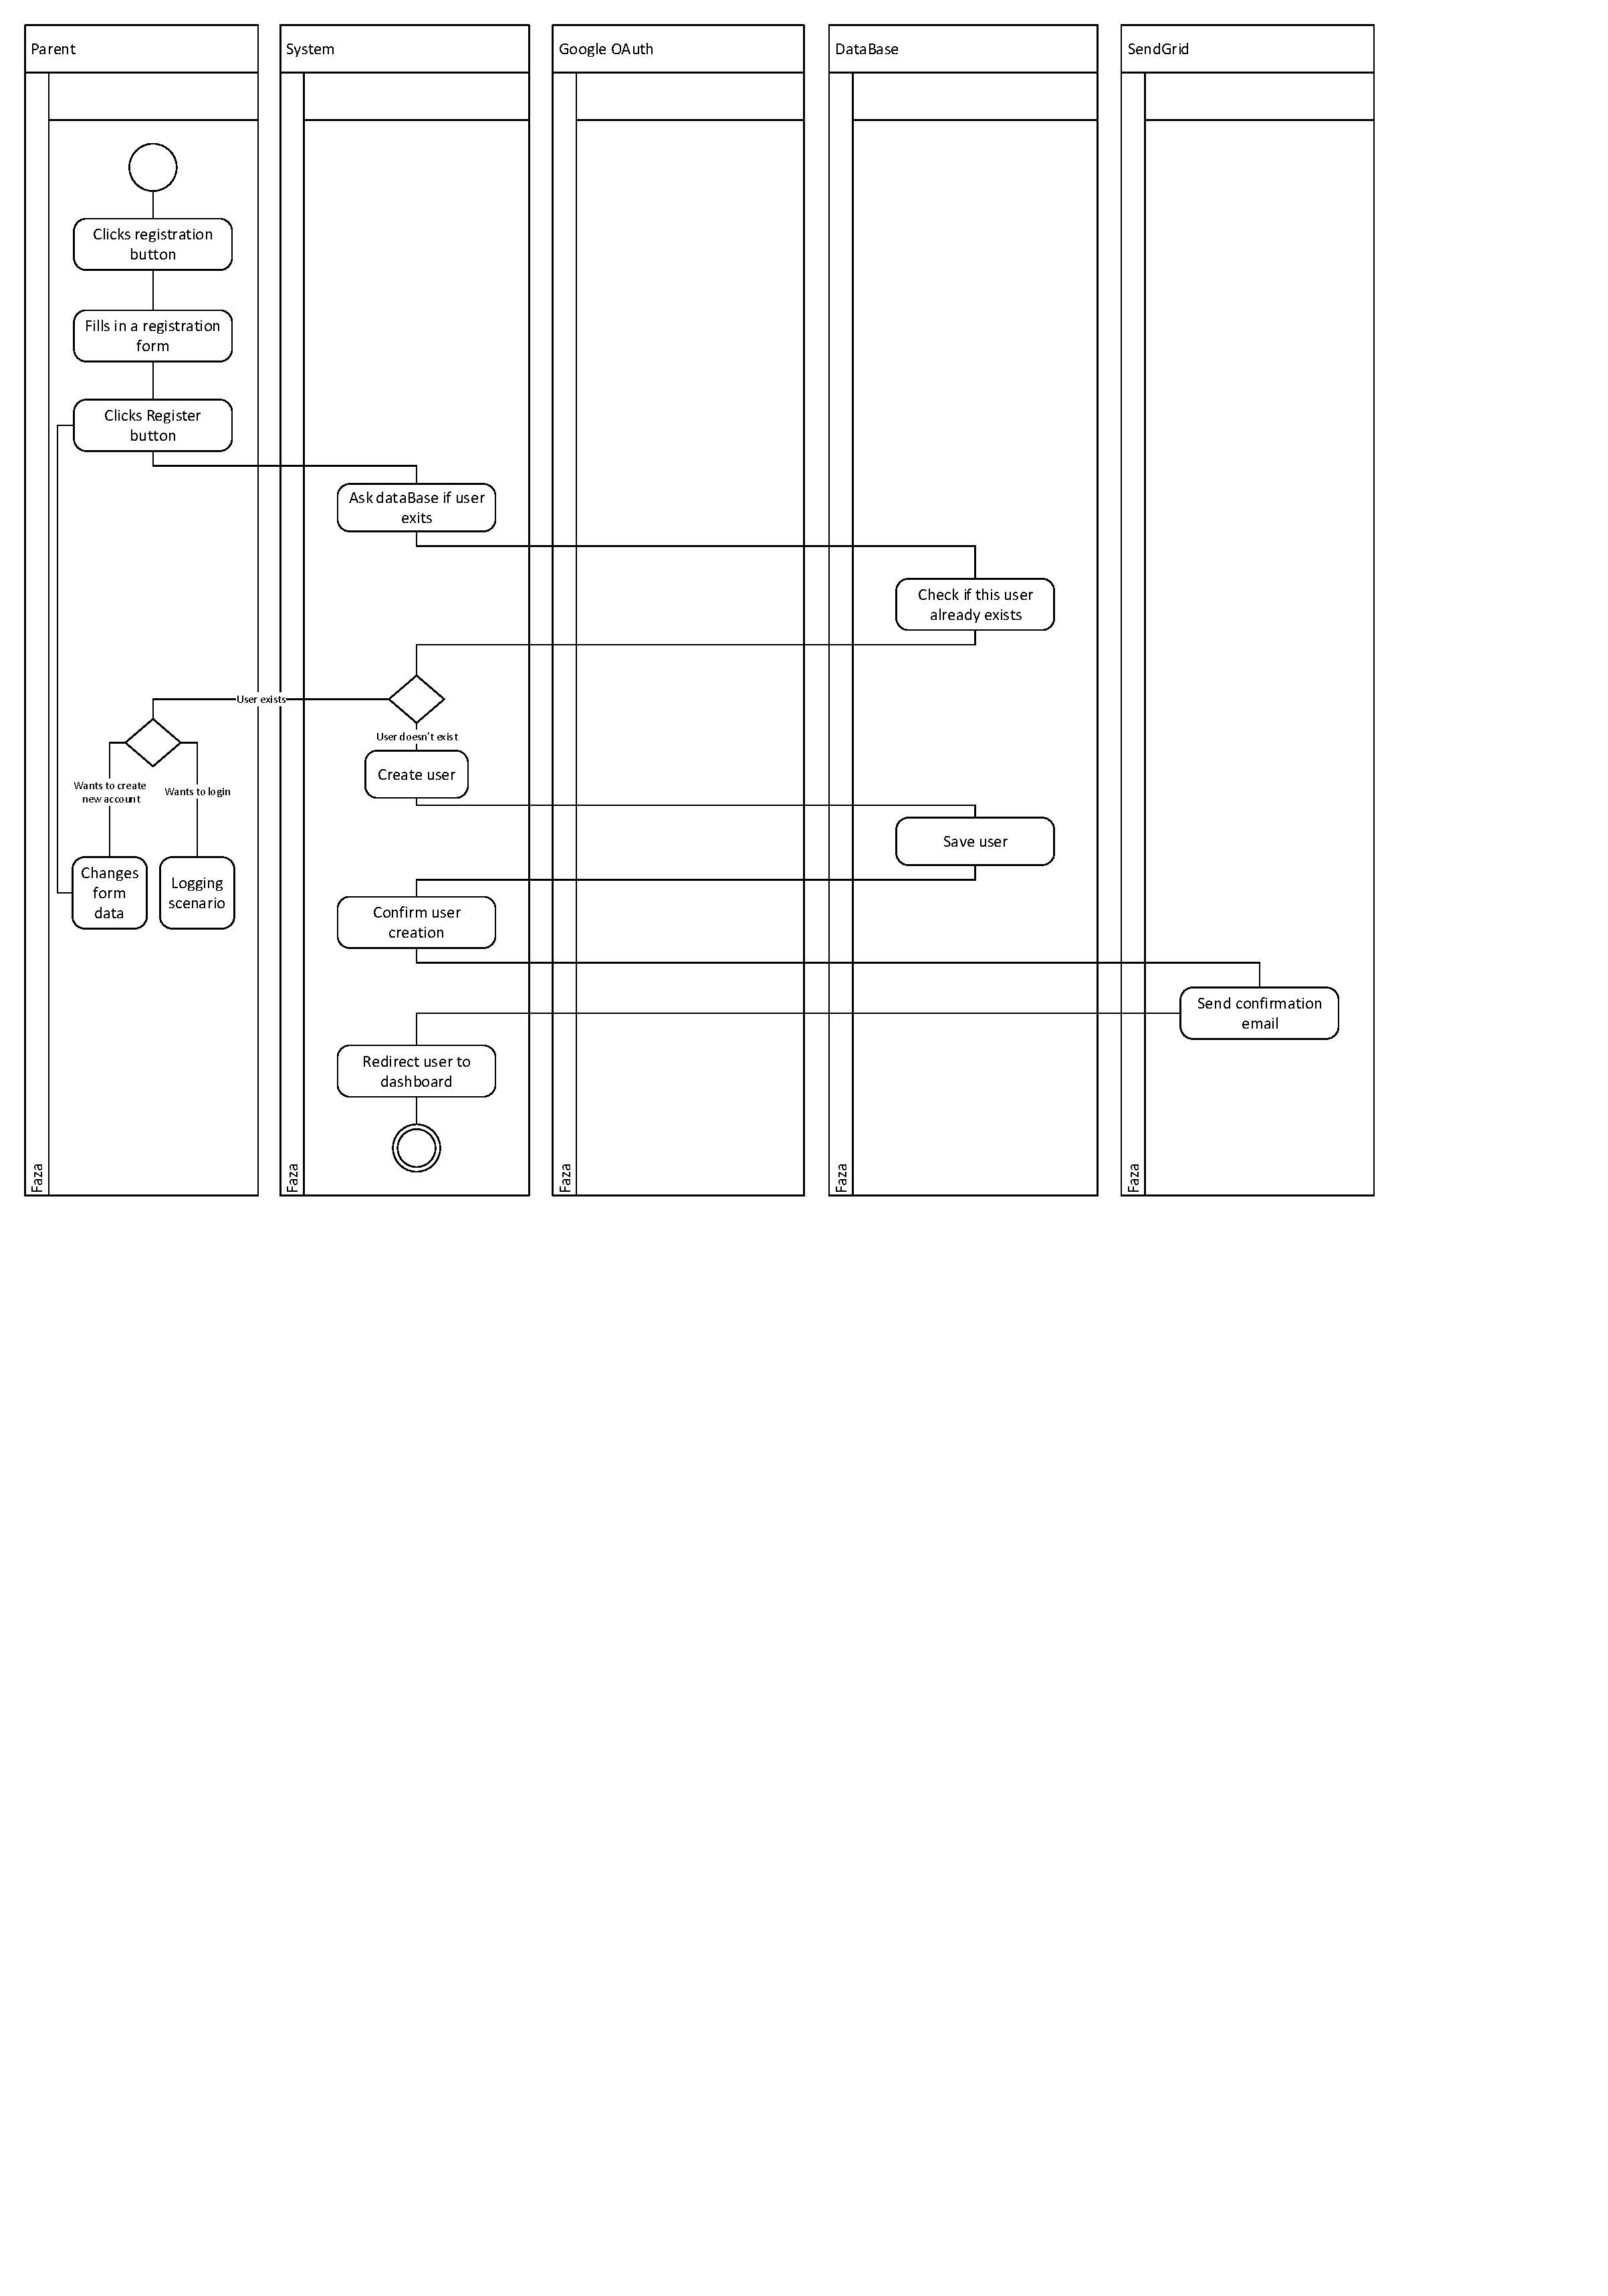
\includegraphics[width=.95\textwidth]{cropped_Registration_Activity_Diagram} 
				\end{tabular}
			\caption{Diagram aktywności dla rejestracji}
			\end{figure}

			\begin{figure}[H]
				\centering
				\begin{tabular}{c}
					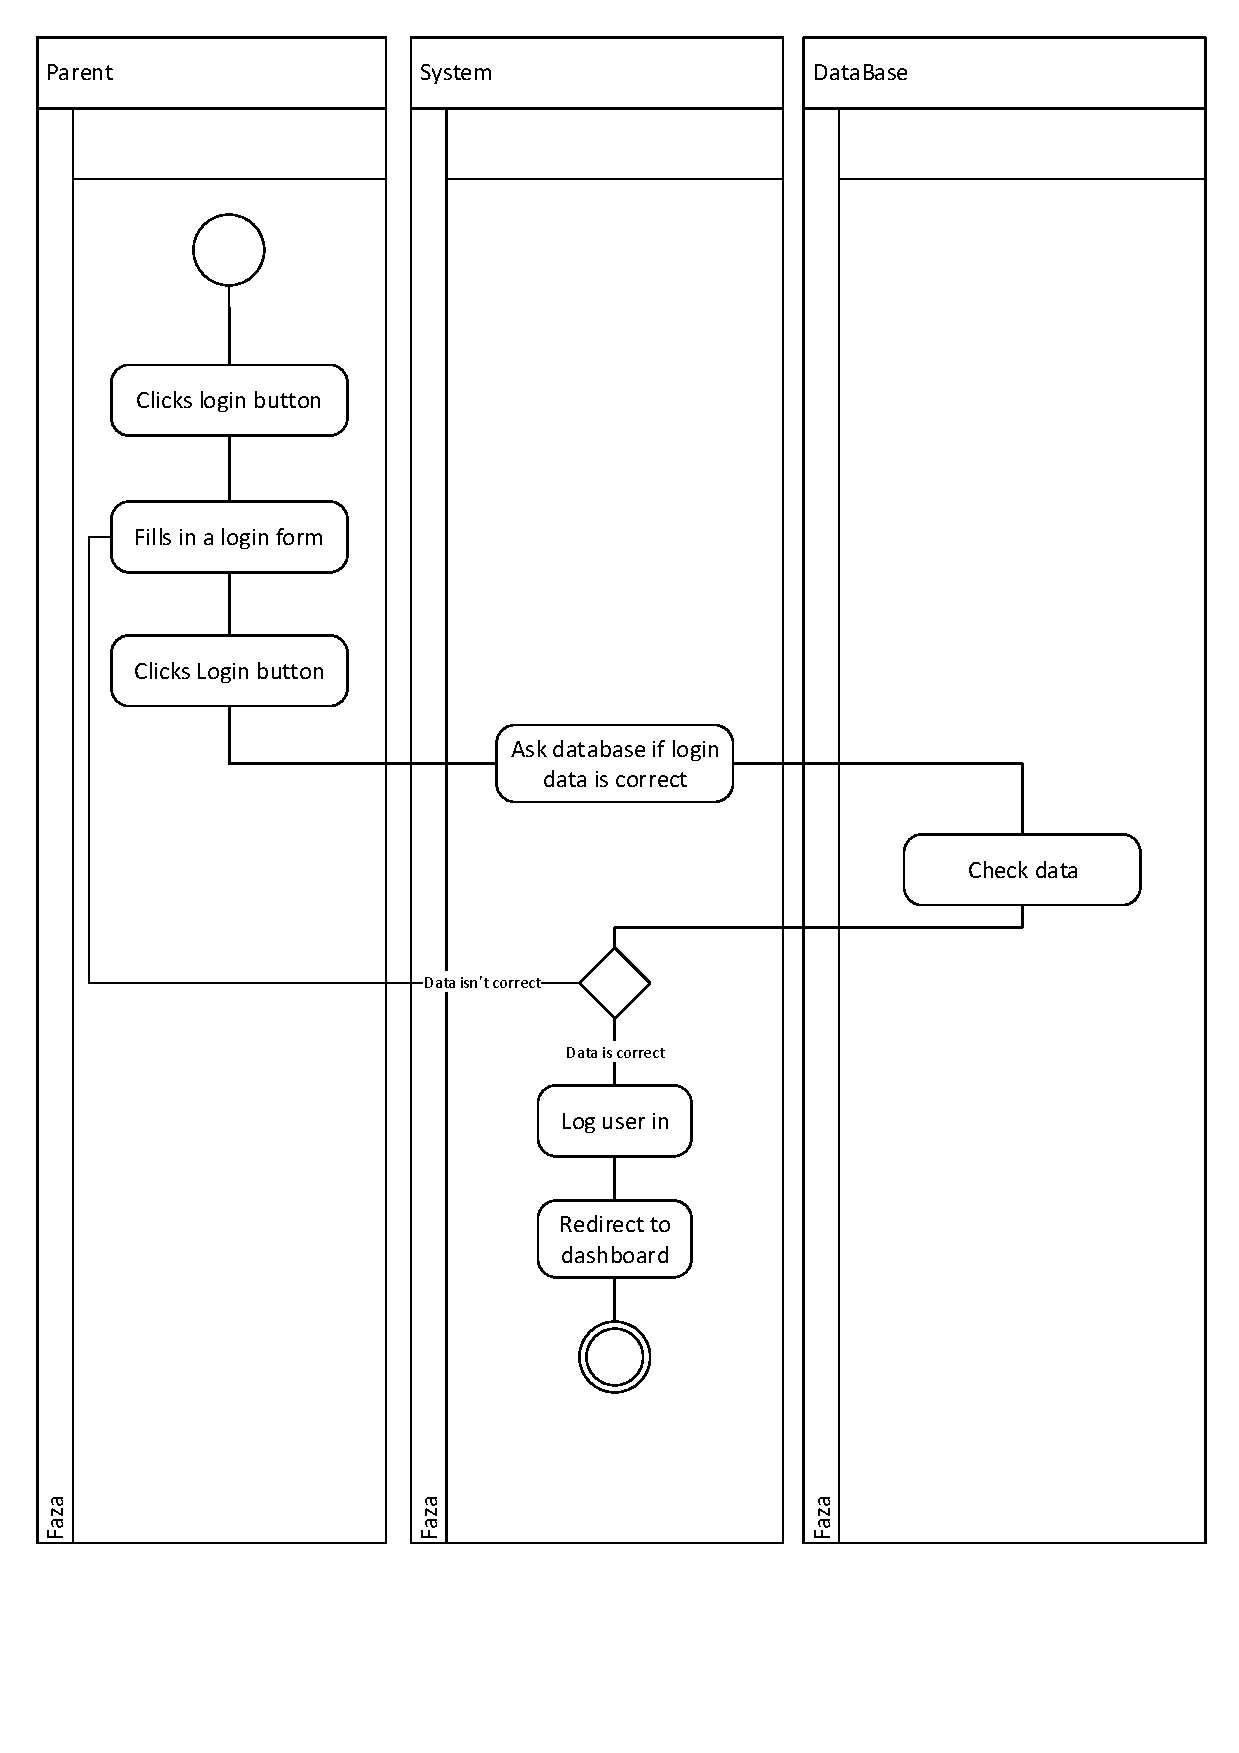
\includegraphics[width=.95\textwidth]{Login_cropped} 
				\end{tabular}
			\caption{Diagram aktywności dla logowania}
			\end{figure}

			\begin{figure}[H]
				\centering
				\begin{tabular}{c}
					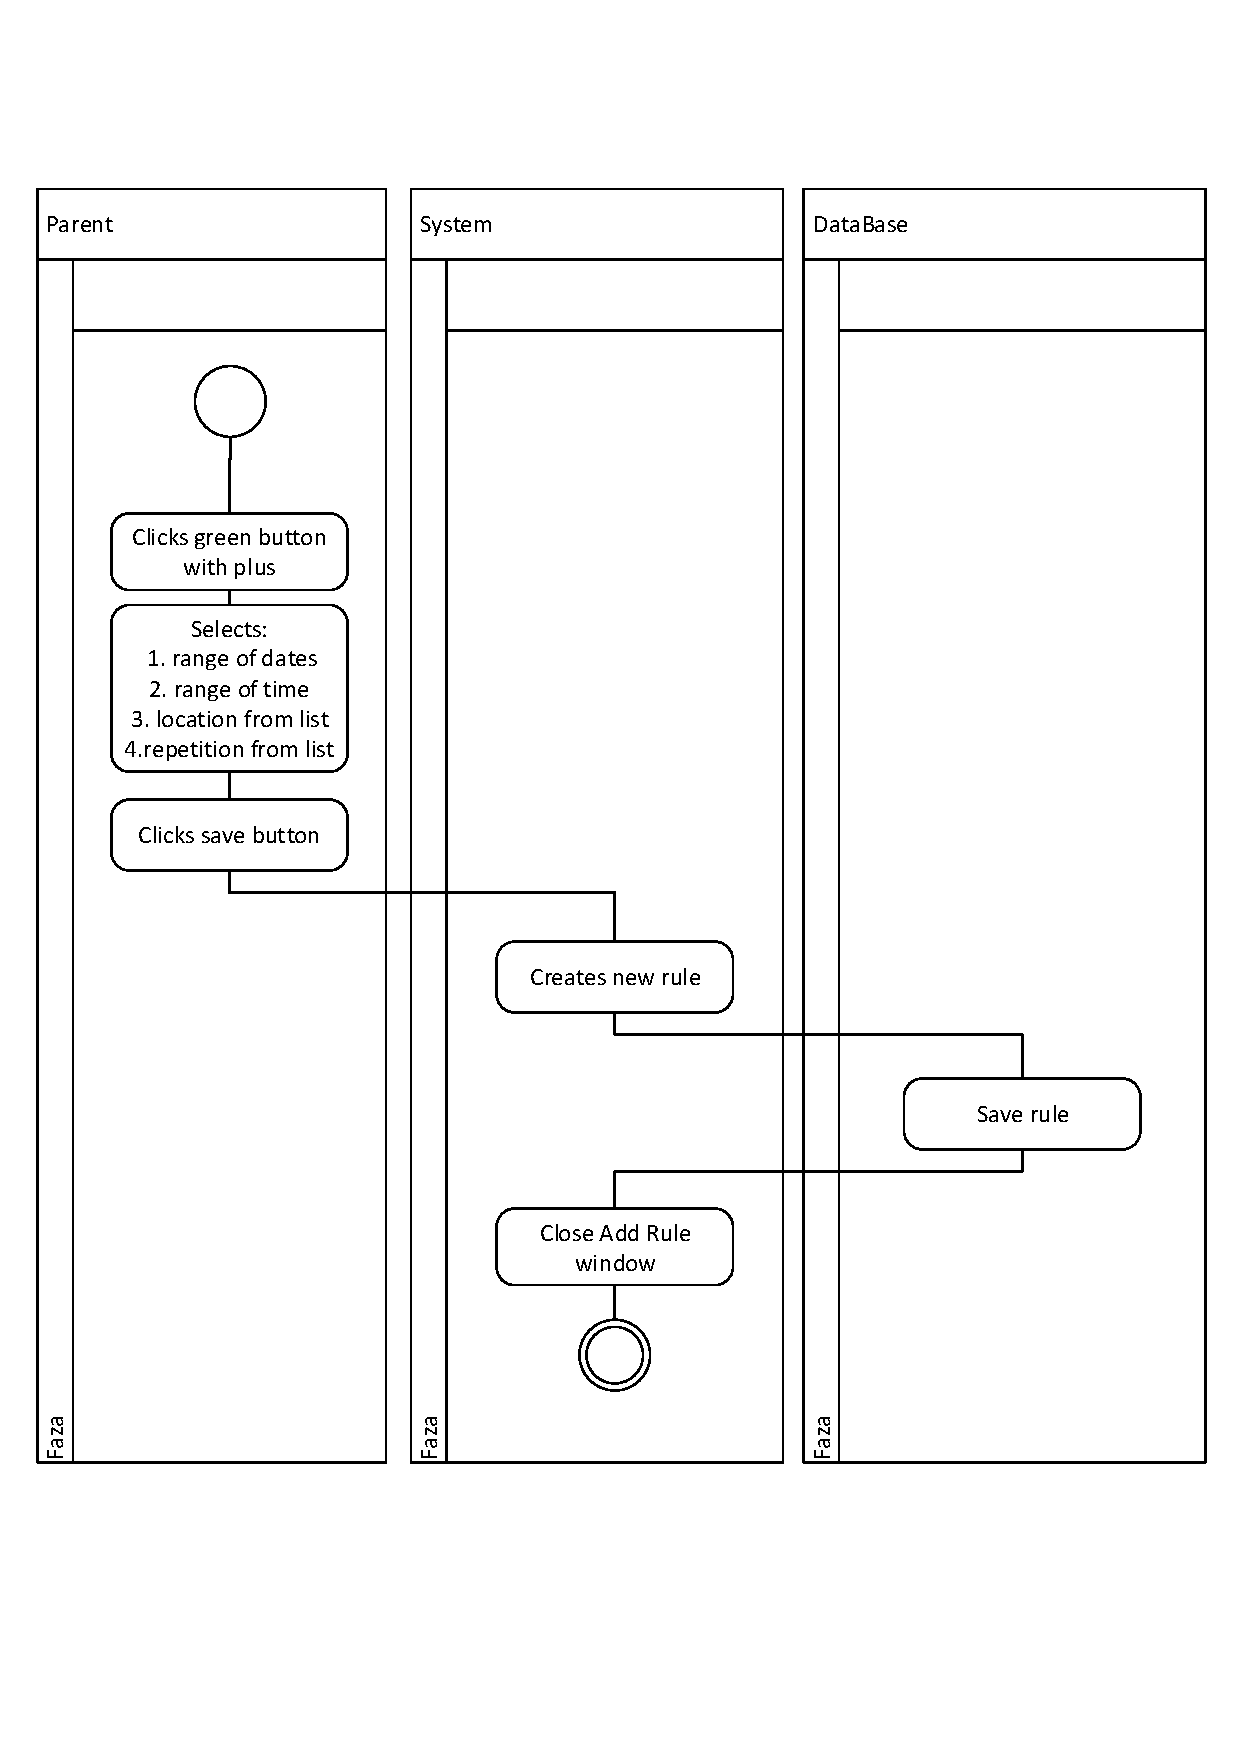
\includegraphics[width=.95\textwidth]{crudCreate_cropped} 
				\end{tabular}
			\caption{Diagram aktywności dla tworzenia nowej reguły}
			\end{figure}

			\begin{figure}[H]
				\centering
				\begin{tabular}{c}
					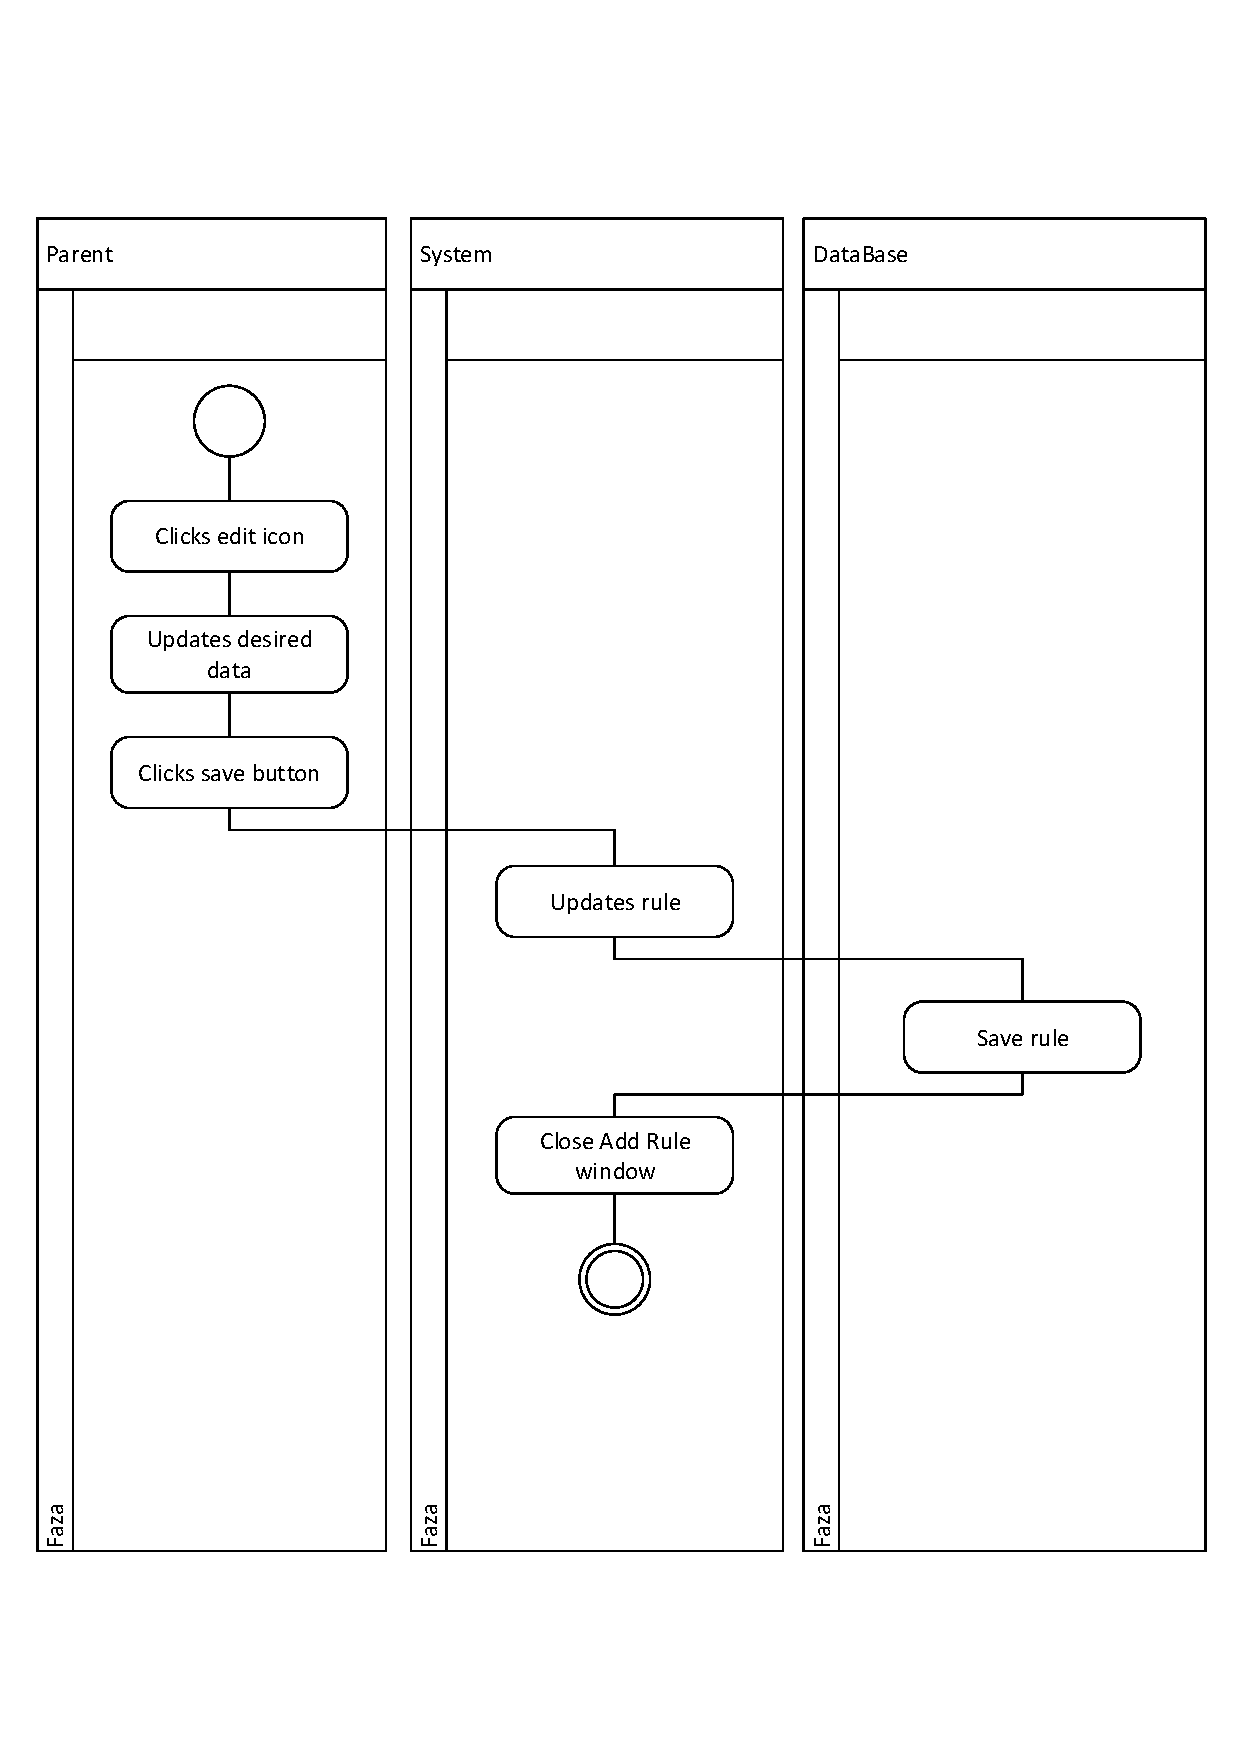
\includegraphics[width=.95\textwidth]{crudUpdate_cropped} 
				\end{tabular}
			\caption{Diagram aktywności dla modyfikacji reguły}
			\end{figure}

			\begin{figure}[H]
				\centering
				\begin{tabular}{c}
					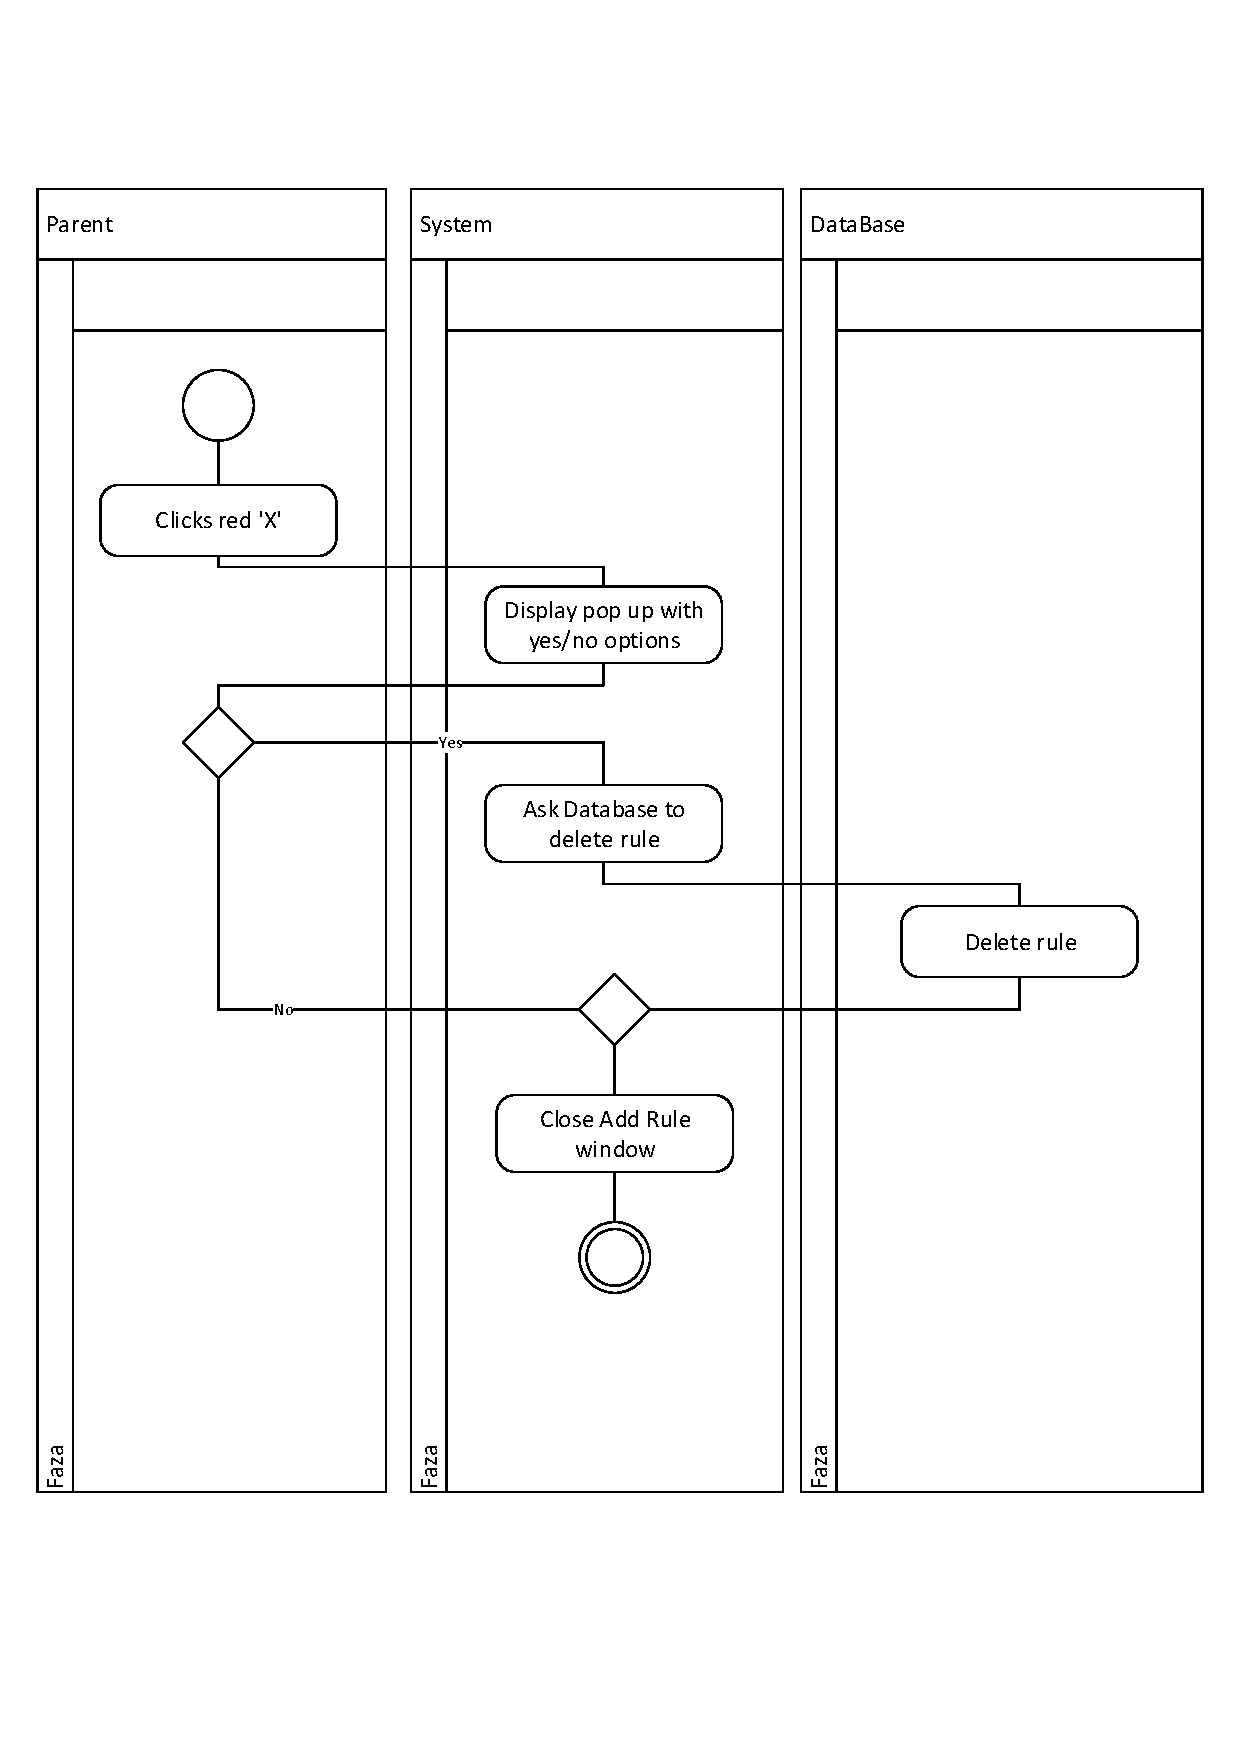
\includegraphics[width=.95\textwidth]{crudDelete_cropped} 
				\end{tabular}
			\caption{Diagram aktywności dla usuwania reguły}
			\end{figure}

			W diagramach wyróżniliśmy operacje CRUD (tworzenie, odczyt, modyfikacja i usuwanie) dla zarządzania regułami. Nie umieszczaliśmy pozostałych, gdyż realizowane są one w analogiczny sposób.

	\section{Analiza dziedziny}

		Klasy zidentyfikowane w aplikacji:
		\begin{itemize}
			\item KontoRodzica - klasa odpowiadająca za przechowywanie informacji o rodzicu takie jak imie, nazwisko, email, suma kontrolna hasła,
			\item KontoDziecka - klasa odpowiadająca za przechowywanie informacji o dziecku takie jak nazwa, email, suma kontrolna hasła,
			\item Reguła - klasa odpowiadająca za przechowywanie informacji o regułach ustalonych dla danego dziecka, dotyczących danego obszaru. Data pierwszego wydarzenia, czas pierwszego wydarzenia, powtarzanie wydarzeń (do wyboru: codziennie, co tydzień, itd.), czas trwania wydarzenia,
			\item Lokalizacja - klasa związana bezpośrednio z klasą KontoDziecka przechowująca lokalizację dziecka. Parametrami jest długość i szerokość geograficzna,
			\item Interfejs Obszaru - klasa interfejsu dla klas Obszarów,
			\item OkrągłyObszar - klasa przechowująca koordynaty X i Y środka okręgu, jego promień opisująca obszar na mapie w którym powinno znajdować się dziecko
		\end{itemize}

		\begin{figure}[H]
			\centering
			\begin{tabular}{c}
				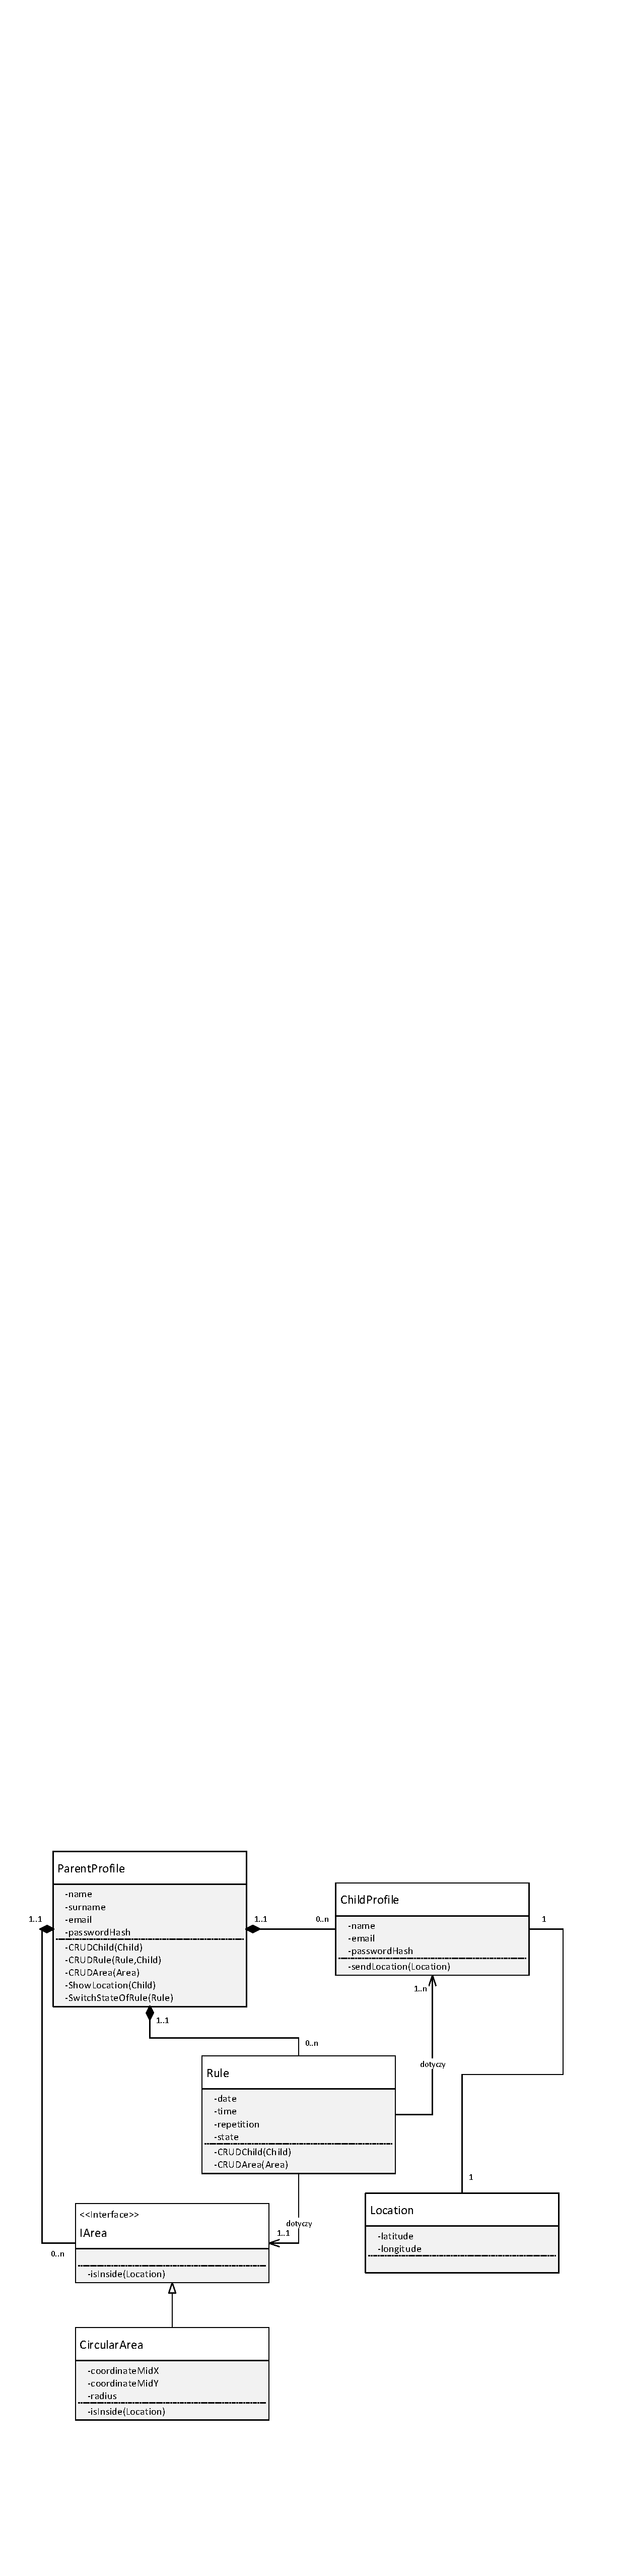
\includegraphics[width=.95\textwidth]{classes} 
			\end{tabular}
		\caption{Diagram klas}
		\end{figure}
	
		\subsection{Diagram stanów dla telefonu dziecka}
		
		\begin{figure}[H]
			\centering
			\begin{tabular}{c}
				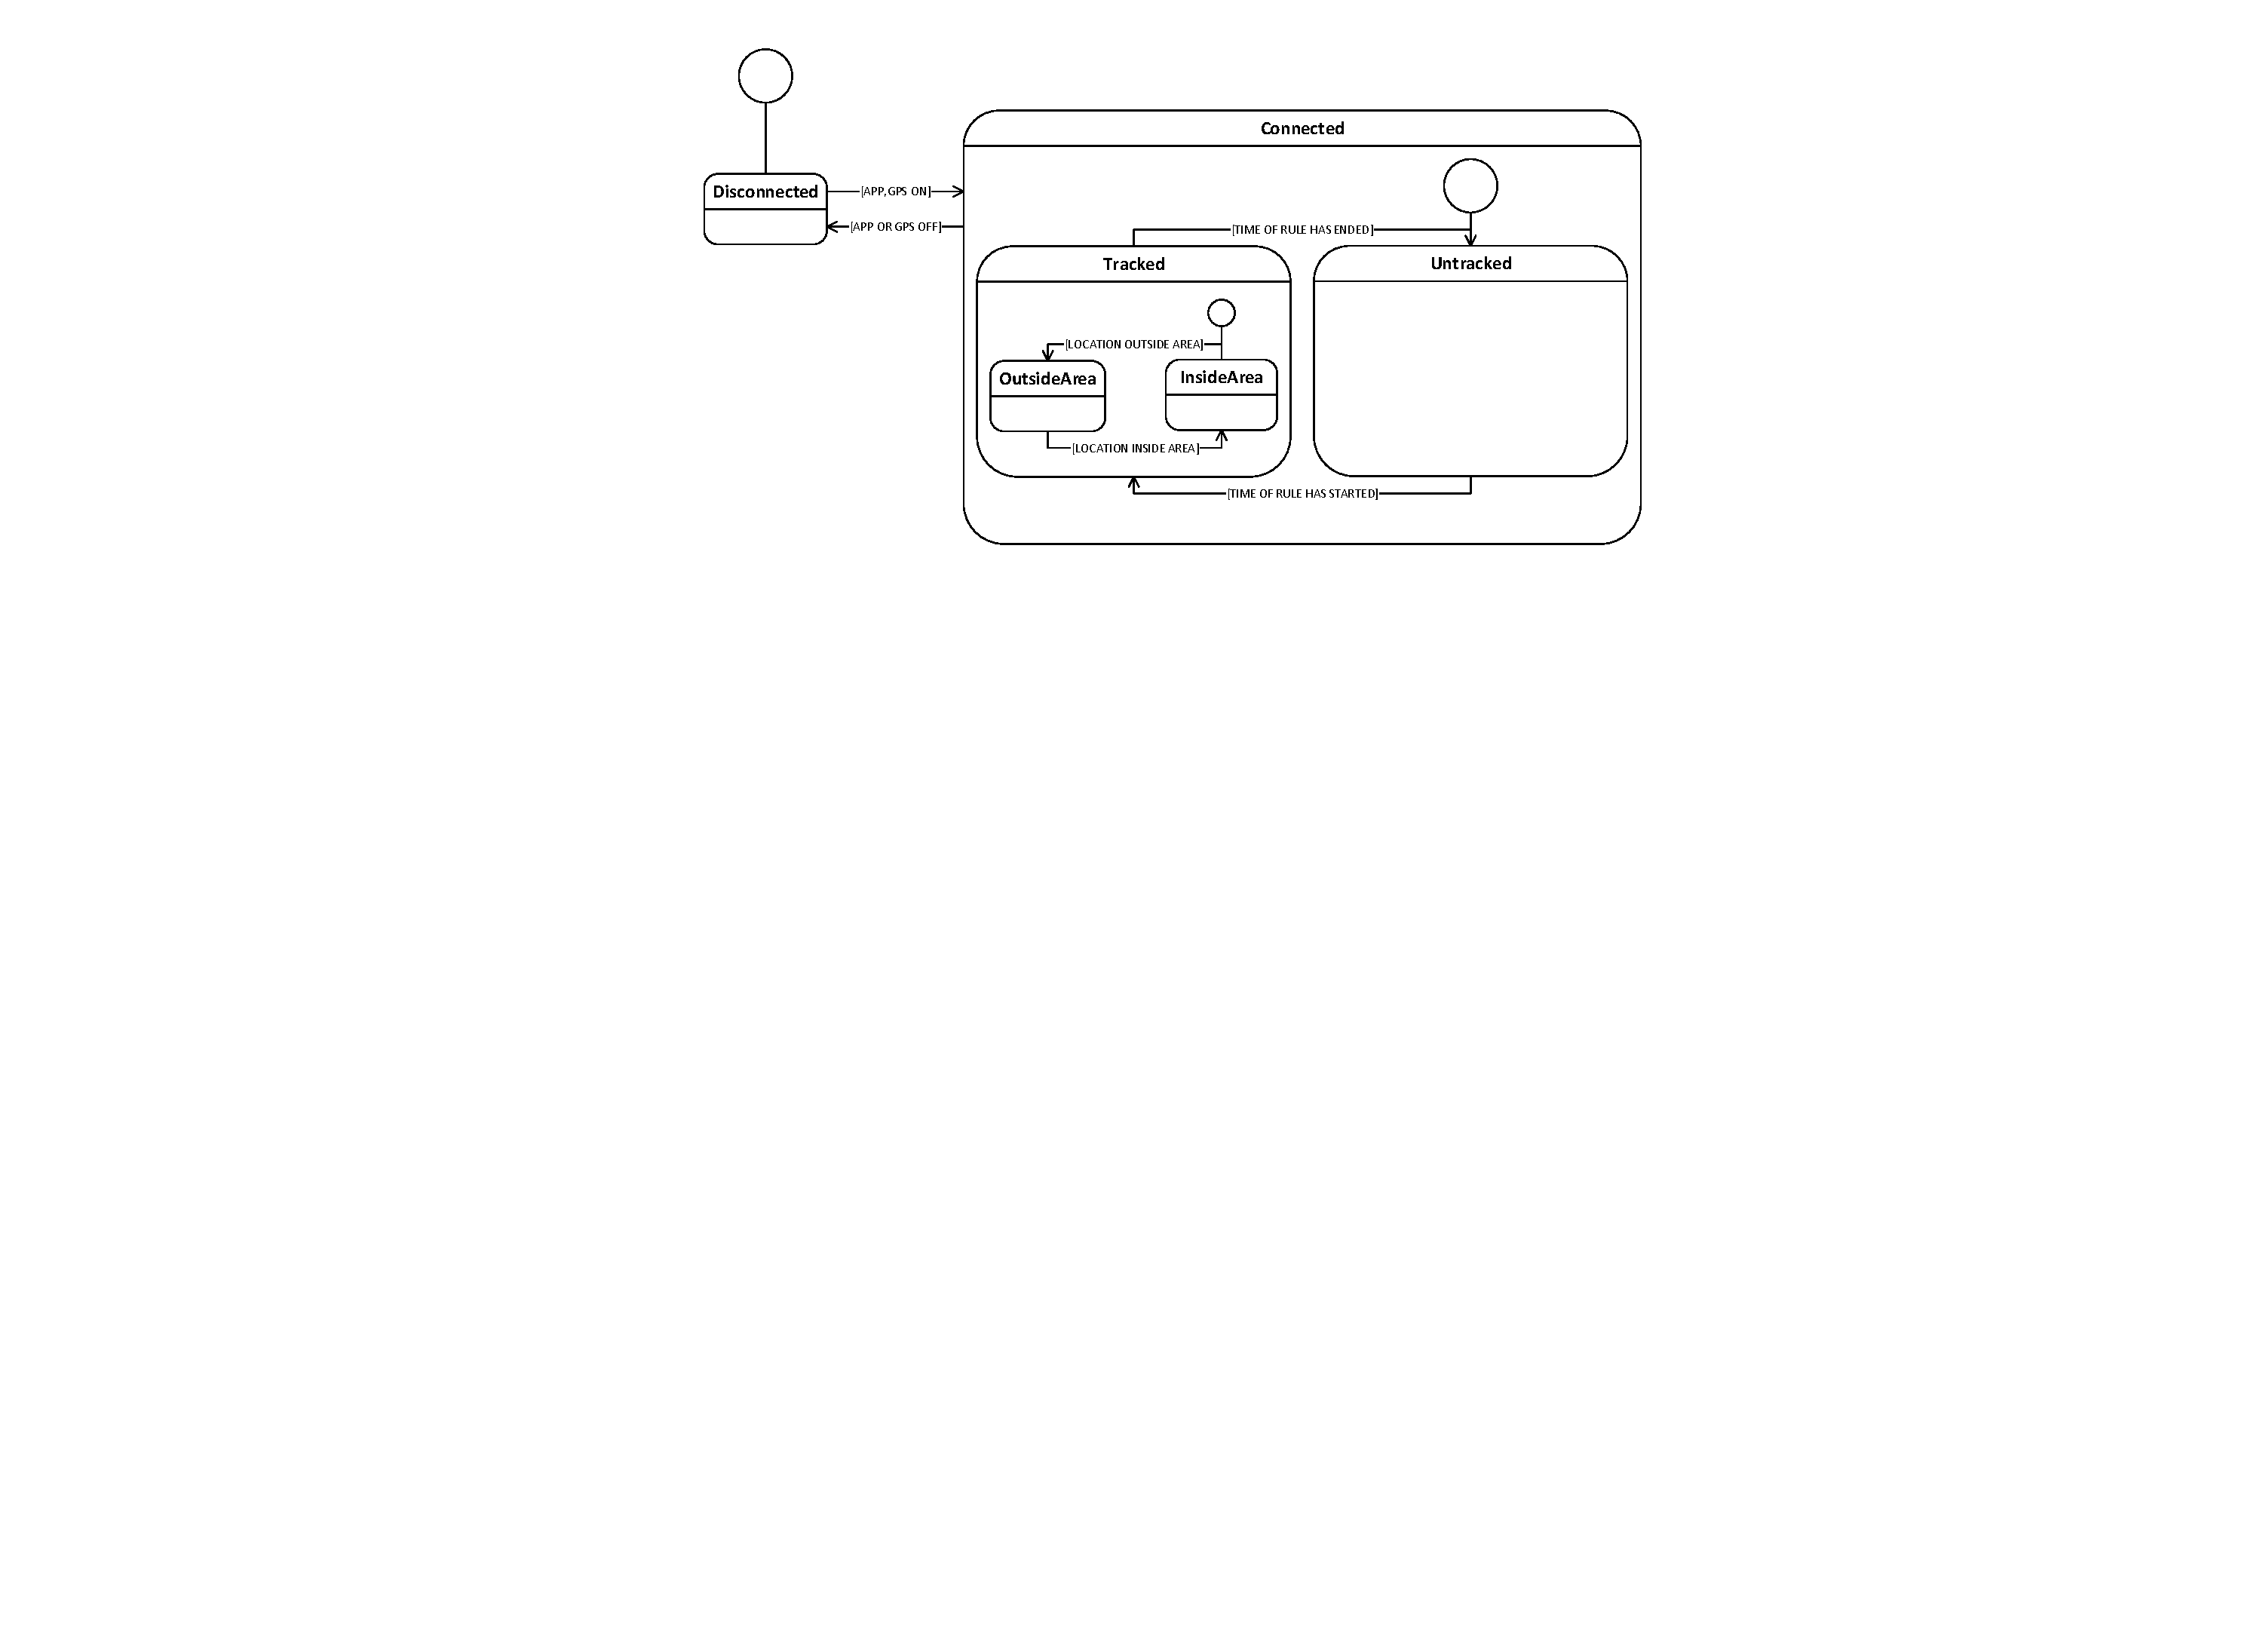
\includegraphics[width=.95\textwidth]{Stanu_cropped} 
			\end{tabular}
			\caption{Diagram stanów}
		\end{figure}

	\section{Specyfikacja wymagań}

		Wymagania stawiane systemowi przedstawione zostały w formie przypadków użycia wraz z scenariuszami.

		\begin{figure}[H]
			\centering
			\begin{tabular}{c}
				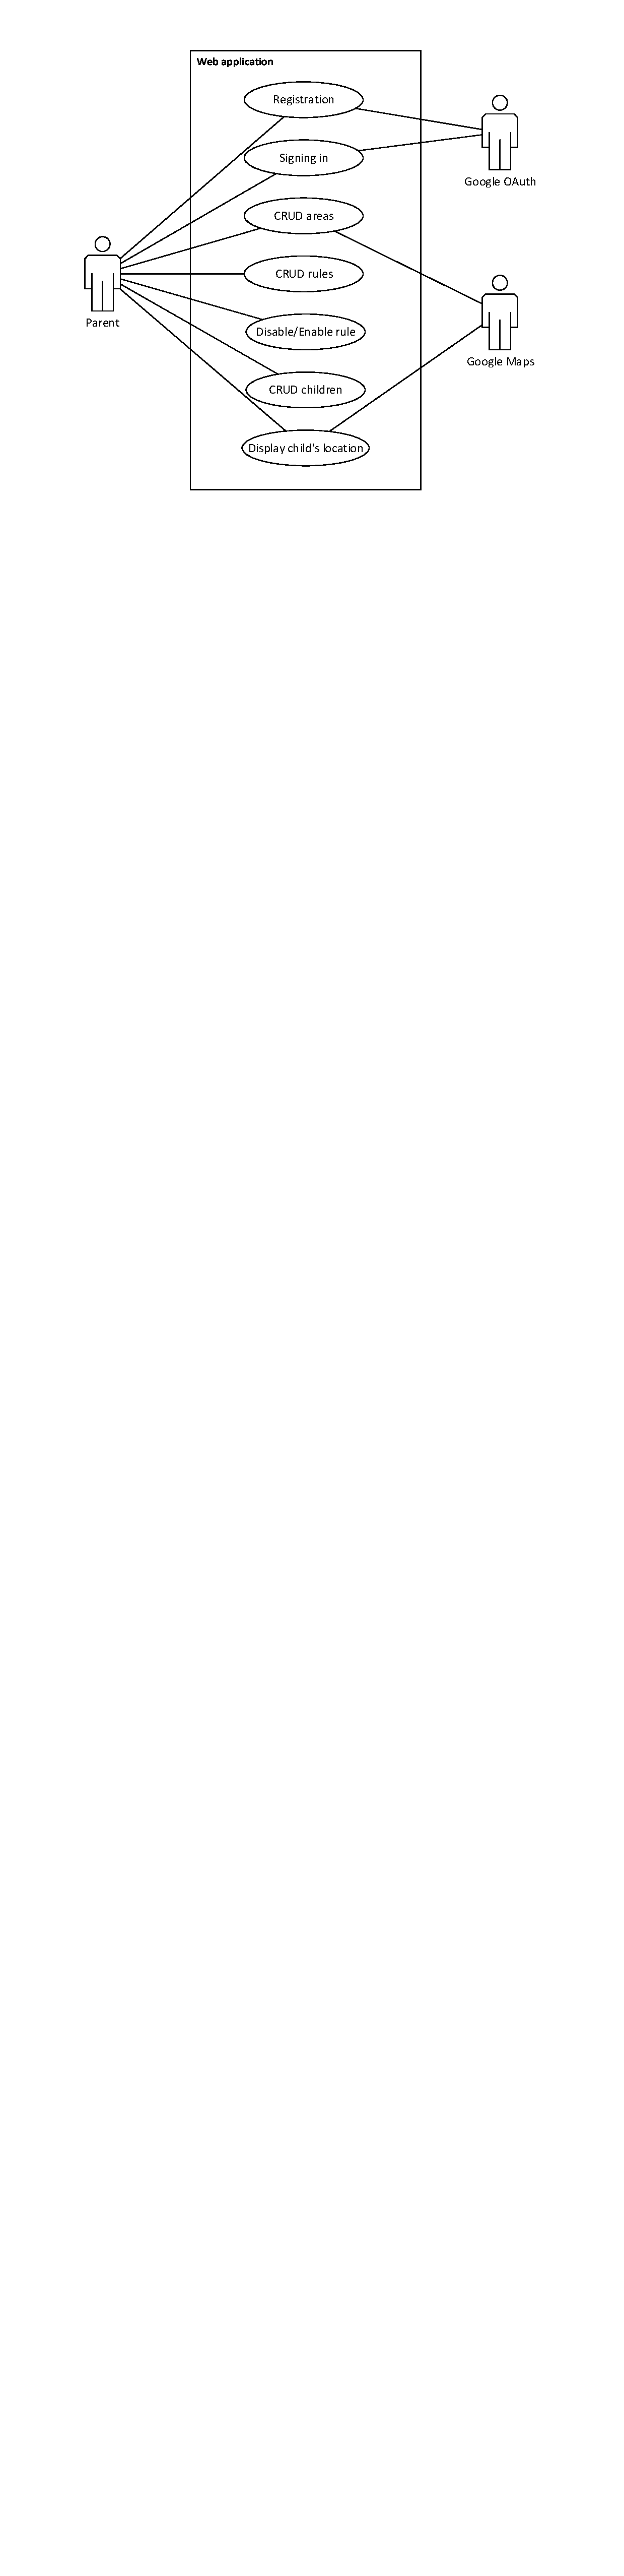
\includegraphics[width=.80\textwidth]{webUseCase} 
			\end{tabular} 
		\caption{Przypadki użycia dla aplikacji webowej}
		\end{figure}

		\begin{figure}[H]
			\centering
			\begin{tabular}{c}
				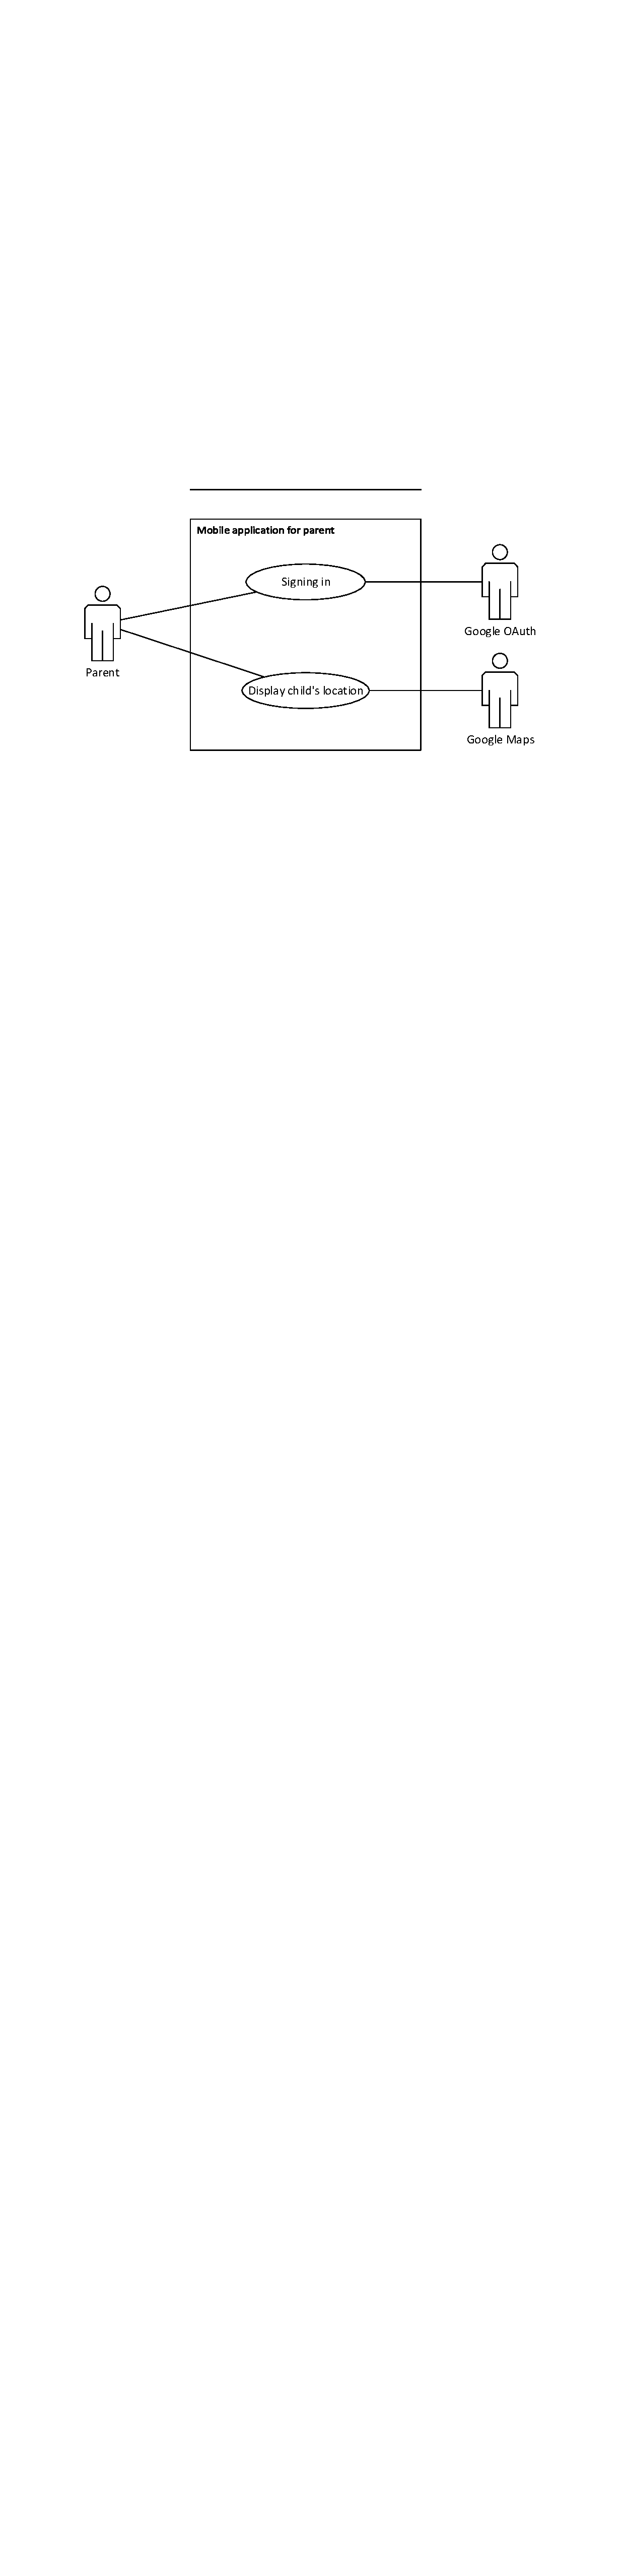
\includegraphics[width=.80\textwidth]{parentUseCase} 
			\end{tabular} 
		\caption{Przypadki użycia dla aplikacji mobilnej rodzica}
		\end{figure} 

		\begin{figure}[H] 
			\centering
			\begin{tabular}{c}
				
\includegraphics[width=.80\textwidth]{childUseCase} 
			\end{tabular} 
		\caption{Przypadki użycia dla aplikacji mobilnej dziecka}
		\end{figure}

		\begin{figure}[H] 
			\centering
			\begin{tabular}{c}
				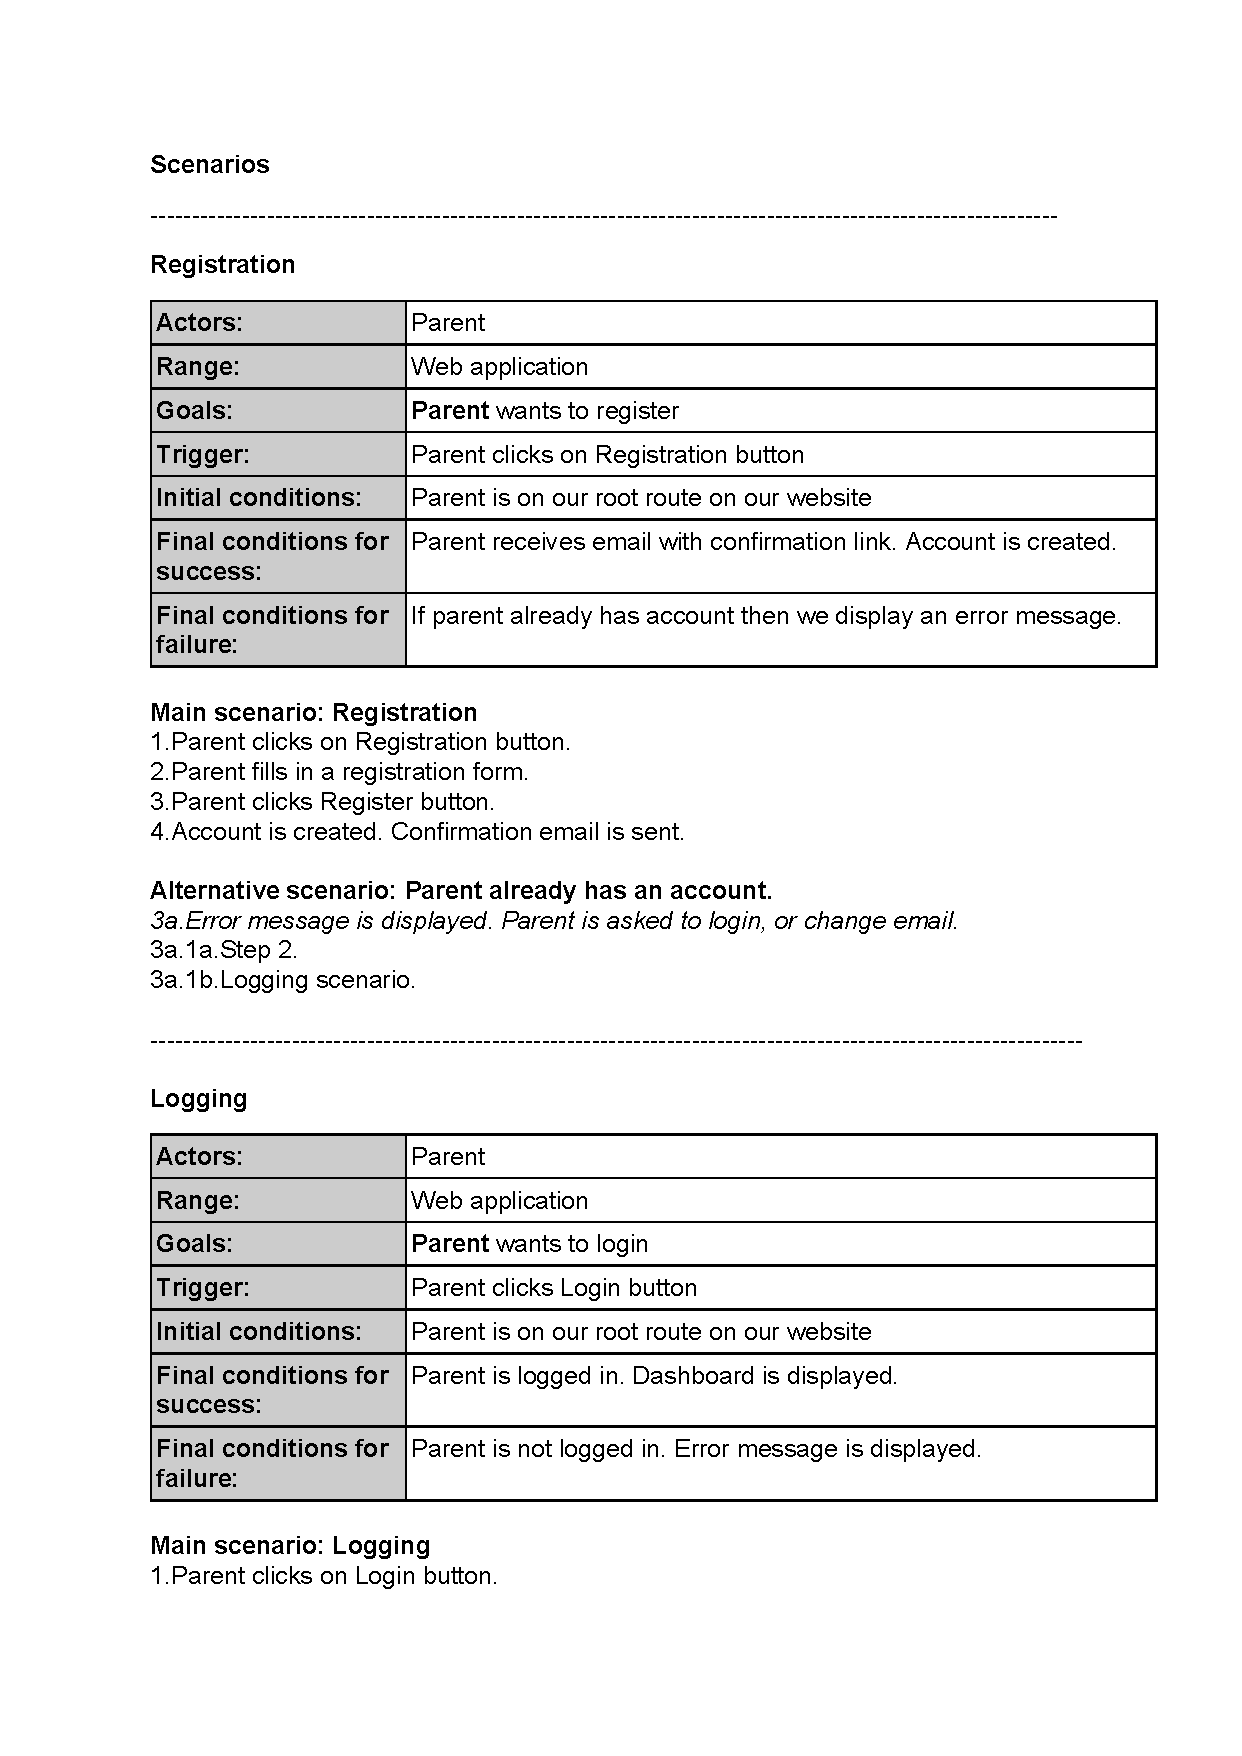
\includegraphics[page=1, width=.95\textwidth]{scenarios} 
			\end{tabular} 
		\end{figure}
		\begin{figure}[H] 
			\centering
			\begin{tabular}{c}
				\includegraphics[page=2, width=.95\textwidth]{scenarios} 
			\end{tabular} 
		\end{figure}
		\begin{figure}[H] 
			\centering
			\begin{tabular}{c}
				\includegraphics[page=3, width=.95\textwidth]{scenarios} 
			\end{tabular} 
		\end{figure}
		\begin{figure}[H] 
			\centering
			\begin{tabular}{c}
				\includegraphics[page=4, width=.95\textwidth]{scenarios} 
			\end{tabular} 
		\end{figure}
		\begin{figure}[H] 
			\centering
			\begin{tabular}{c}
				\includegraphics[page=5, width=.95\textwidth]{scenarios} 
			\end{tabular} 
		\end{figure}
		\begin{figure}[H] 
			\centering
			\begin{tabular}{c}
				\includegraphics[page=6, width=.95\textwidth]{scenarios} 
			\end{tabular} 
		\end{figure}
		

	\section{Architektura systemu}
		Do zaimplementowania bazy danych skorzystaliśmy z MongoDB, dlatego schemat bazy będzie idealnym odwzorowaniem diagramu klas dla aplikacji.
		
		\begin{figure}[H] 
			\centering
			\begin{tabular}{c}
				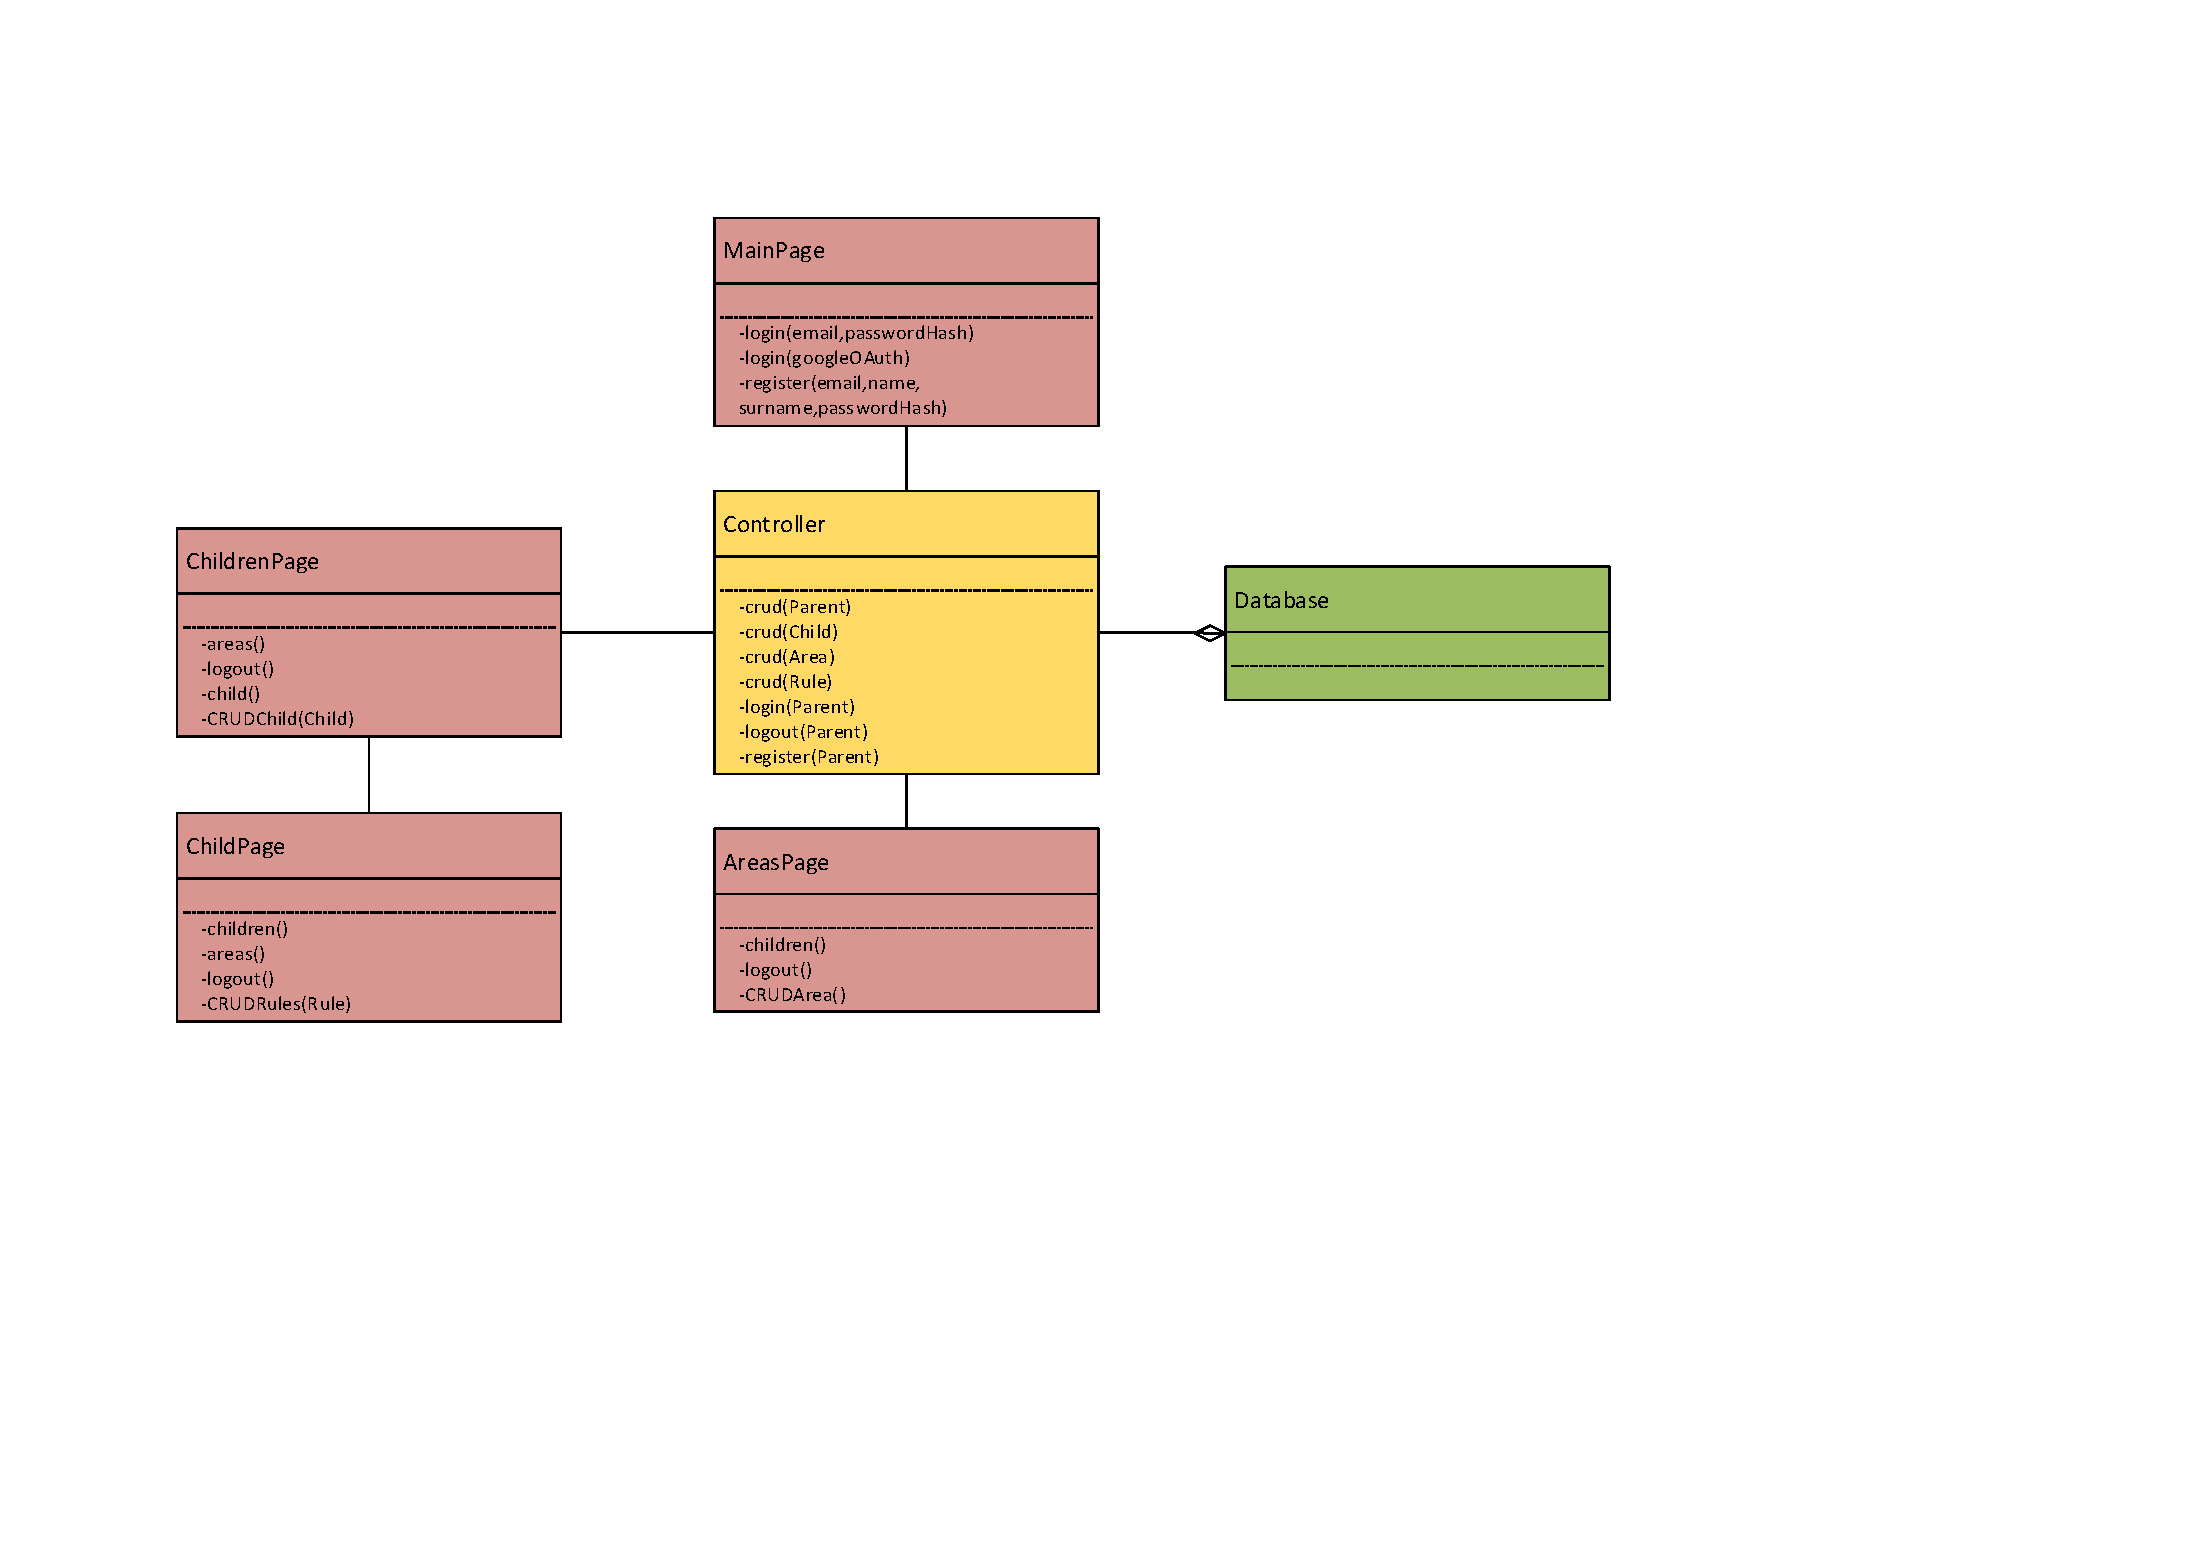
\includegraphics[width=.95\textwidth]{MVC_cropped} 
			\end{tabular} 
			\caption{Diagram implementacji modelu MVC}
		\end{figure}

		Komunikacja w aplikacji będzie obsługiwana przez serwer, który udostępnia api. Użytkownik poprzez wypełnianie różnych formularzy, czy klikanie przycisków, będzie wysyłał zapytania do serwera. Serwer uruchomi odpowiednie działanie na bazie danych i zwróci właściwą odpowiedź. Na podstawie informacji z serwera komponenty strony zaktualizują się lub użytkownik zostanie przekierowany na odpowiedni adres.
		
		\subsection{Opis API}
		\begin{itemize}
			\item \textbackslash api\textbackslash current\_user - zwraca bieżącego użytkownika, aby kontrolować czy użytkownik jest zalogowany,
			\item \textbackslash api\textbackslash logout - wylogowuje użytkownika,
			\item \textbackslash api\textbackslash googleAuth - logowanie z Google,
			\item \textbackslash api\textbackslash register - rejestrowanie nowych użytkowników,
			\item \textbackslash api\textbackslash login - logowanie użytkowników,
			
			\item \textbackslash api\textbackslash rules - pobieranie reguł dla danego rodzica
			\item \textbackslash api\textbackslash rules\textbackslash create - dodawanie reguły
			\item \textbackslash api\textbackslash rules\textbackslash read - odczyt reguły
			\item \textbackslash api\textbackslash rules\textbackslash update - modyfikowanie reguły
			\item \textbackslash api\textbackslash rules\textbackslash delete - usuwanie reguły
			
			\item \textbackslash api\textbackslash areas - pobieranie obszarów dla danego rodzica
			\item \textbackslash api\textbackslash areas\textbackslash create - dodawanie obszaru
			\item \textbackslash api\textbackslash areas\textbackslash read - odczyt obszaru
			\item \textbackslash api\textbackslash areas\textbackslash update - modyfikowanie obszaru
			\item \textbackslash api\textbackslash areas\textbackslash delete - usuwanie obszaru
			
			\item \textbackslash api\textbackslash children - pobieranie dzieci dla danego rodzica
			\item \textbackslash api\textbackslash children\textbackslash create - dodawanie dziecka
			\item \textbackslash api\textbackslash children\textbackslash read - odczyt dziecka
			\item \textbackslash api\textbackslash children\textbackslash update - modyfikowanie dziecka
			\item \textbackslash api\textbackslash children\textbackslash delete - usuwanie dziecka
			
		\end{itemize}
		

	\section{Projekt oprogramowania}
	
		\begin{figure}[H] 
			\centering
			\begin{tabular}{c}
				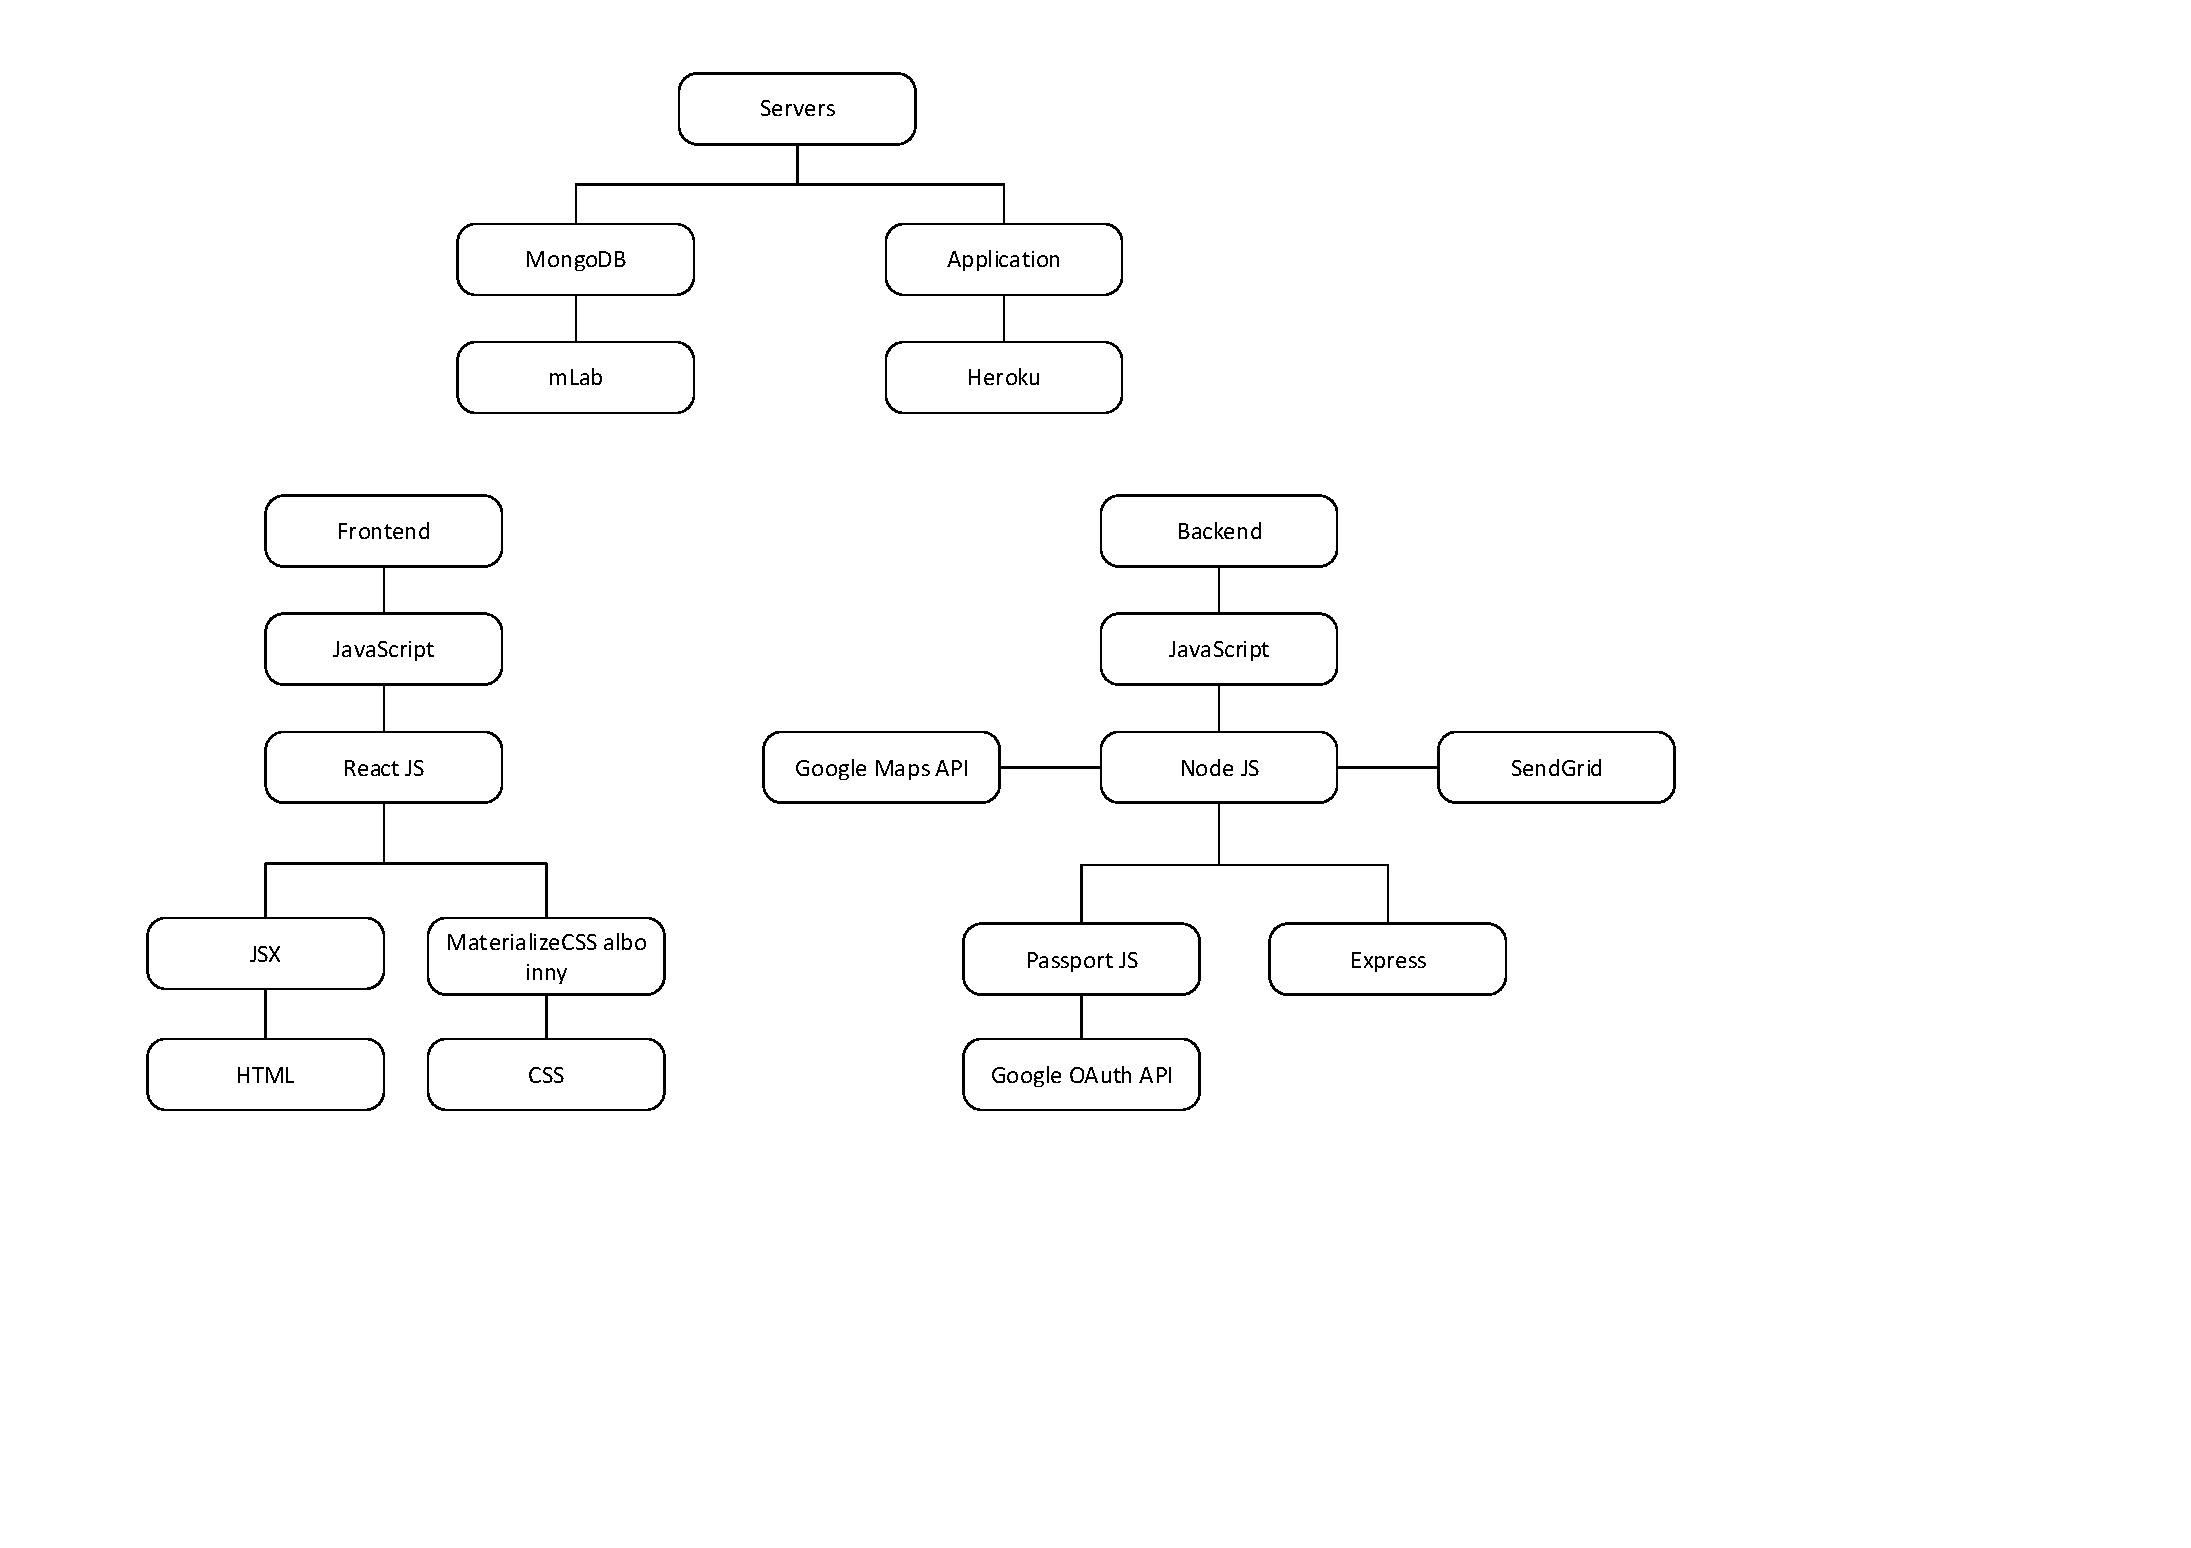
\includegraphics[width=.95\textwidth]{Stos_cropped} 
			\end{tabular} 
			\caption{Stos technologiczny}
		\end{figure}

	\section{Projekt interfejsu użytkownika}

		\begin{figure}[H] 
			\centering
			\begin{tabular}{c}
				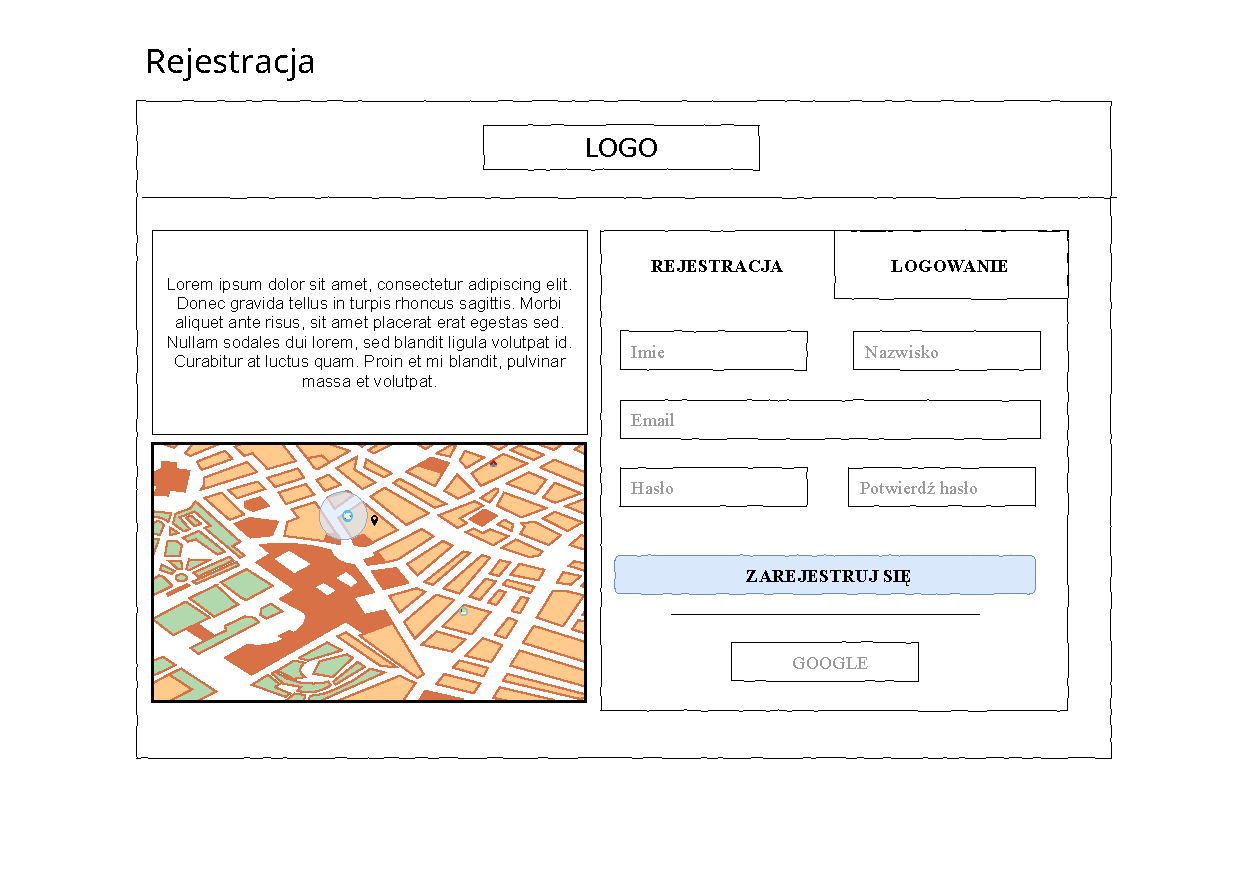
\includegraphics[page=1, width=.95\textwidth]{Interfejs_Web} 
			\end{tabular} 
		\end{figure}
		\begin{figure}[H] 
			\centering
			\begin{tabular}{c}
				\includegraphics[page=2, width=.95\textwidth]{Interfejs_Web} 
			\end{tabular} 
		\end{figure}
		\begin{figure}[H] 
			\centering
			\begin{tabular}{c}
				\includegraphics[page=3, width=.95\textwidth]{Interfejs_Web} 
			\end{tabular} 
		\end{figure}
		\begin{figure}[H] 
			\centering
			\begin{tabular}{c}
				\includegraphics[page=4, width=.95\textwidth]{Interfejs_Web} 
			\end{tabular} 
		\end{figure}
		\begin{figure}[H] 
			\centering
			\begin{tabular}{c}
				\includegraphics[page=5, width=.95\textwidth]{Interfejs_Web} 
			\end{tabular} 
		\end{figure}
		\begin{figure}[H] 
			\centering
			\begin{tabular}{c}
				\includegraphics[page=6, width=.95\textwidth]{Interfejs_Web} 
			\end{tabular} 
		\end{figure}
		\begin{figure}[H] 
			\centering
			\begin{tabular}{c}
				\includegraphics[page=7, width=.95\textwidth]{Interfejs_Web} 
			\end{tabular} 
		\end{figure}
		\begin{figure}[H] 
			\centering
			\begin{tabular}{c}
				\includegraphics[page=8, width=.95\textwidth]{Interfejs_Web} 
			\end{tabular} 
		\end{figure}
		\begin{figure}[H] 
			\centering
			\begin{tabular}{c}
				\includegraphics[page=9, width=.95\textwidth]{Interfejs_Web} 
			\end{tabular} 
		\end{figure}
		\begin{figure}[H] 
			\centering
			\begin{tabular}{c}
				\includegraphics[page=10, width=.95\textwidth]{Interfejs_Web} 
			\end{tabular} 
		\end{figure}
		\begin{figure}[H] 
			\centering
			\begin{tabular}{c}
				\includegraphics[page=11, width=.95\textwidth]{Interfejs_Web} 
			\end{tabular} 
		\end{figure}
		\begin{figure}[H] 
			\centering
			\begin{tabular}{c}
				\includegraphics[page=12, width=.95\textwidth]{Interfejs_Web} 
			\end{tabular} 
		\end{figure}
		\begin{figure}[H] 
			\centering
			\begin{tabular}{c}
				\includegraphics[page=13, width=.95\textwidth]{Interfejs_Web} 
			\end{tabular} 
		\end{figure}
		\begin{figure}[H] 
			\centering
			\begin{tabular}{c}
				\includegraphics[page=14, width=.95\textwidth]{Interfejs_Web} 
			\end{tabular} 
		\end{figure}
		\begin{figure}[H] 
			\centering
			\begin{tabular}{c}
				\includegraphics[page=15, width=.95\textwidth]{Interfejs_Web} 
			\end{tabular} 
		\end{figure}
		\begin{figure}[H] 
			\centering
			\begin{tabular}{c}
				\includegraphics[page=16, width=.95\textwidth]{Interfejs_Web} 
			\end{tabular} 
		\end{figure}
		\begin{figure}[H] 
			\centering
			\begin{tabular}{c}
				\includegraphics[page=17, width=.95\textwidth]{Interfejs_Web} 
			\end{tabular} 
		\end{figure}

\end{document}